% ----------------------------------------------------------------------------
% File: analyse.tex
% Usage:        Latex2e
% Creation :  19-1-2011 morvan@enib.fr
% Revised:    
% Revised:   
% ----------------------------------------------------------------------------
\documentclass[12pt, a4paper]{book}
% ----------------------------------------------------------------------------
%-------------------------------------------------------------------------
\usepackage{helvet}
\usepackage[francais]{babel}
\usepackage[latin1]{inputenc}
\usepackage{moreverb}
\usepackage{eurosym}
\usepackage{index}
\usepackage{amsfonts}
\usepackage{graphics}
\usepackage{listings}
\usepackage{hyperref}
%\usepackage{html}
\usepackage{multimedia}
\usepackage{pgfpages}
\usepackage{pgf,xcolor,tikz}
\usepackage{rotating}
\usepackage{framed}
\usepackage[framed,hyperref,standard]{ntheorem}
\usepackage{fancyhdr,lastpage}
\usepackage{fancyvrb}

%-------------------------------------------------------------------------
% --- Commandes --------------------------------------------------------------
\renewcommand{\chaptermark}[1]{\markboth{#1}{}}

\renewcommand\contentsname{Table des mati\`eres}
\def\ladate{novembre 2018}
\def\mot-cle#1{
	{\noindent {\bf Mots-cl\'es} : #1\vspace{-.5em}\vspace{0pt}}
	\def\mot-cle{\par}
}

\def\biblio#1{\subsection{R\'ef\'erences}\list
	{[\arabic{enumi}]}{\settowidth\labelwidth{[#1]}\leftmargin\labelwidth
		\advance\leftmargin\labelsep
		\usecounter{enumi}}
	\def\newblock{\hskip .11em plus .33em minus .07em}
	\sloppy\clubpenalty4000\widowpenalty4000
	\sfcode`\.=1000\relax}
\let\endbiblio=\endlist


% --- Identification du document ---------------------------------------------
\def\soustitre{\bf\sc Impression de donn�es maritimes en 3D}
\def\projet{\bf\sc NaVisu}
\def\sousprojet{\bf\sc Dossier de d�veloppement}
\def\titre{\bf\sc NaVisu }
\def\auteur{\sc{Lithops}}
\def\leclient{Projet Open Source}
\def\lauteur{Lithops}
\def\leverif{l}
\def\chef{Lithops}
\def\lechef{sm}
\def\laversion{2.0}
\def\sujet{\sc Manuel d�veloppeur} 

% --- Mise en page ------------------------------------------------------------
\setlength{\textwidth}{17.5cm}
\setlength{\textheight}{24.6cm}
\headsep=2cm
\footskip=1.5cm
\hoffset=-2cm
\voffset=-2.5cm
%--------------------------------------------------------------------------
% Changement de la syntaxe de la commande \chapter

\makeatletter 

%-------------------------------------------------------------------------
\hypersetup{
	bookmarks=true,         % show bookmarks bar?
	unicode=false,          % non-Latin characters in Acrobat�s bookmarks
	pdftoolbar=true,        % show Acrobat�s toolbar?
	pdfmenubar=true,        % show Acrobat�s menu?
	pdffitwindow=false,     % window fit to page when opened
	pdfstartview={FitH},    % fits the width of the page to the window
	pdftitle={My title},    % title
	pdfauthor={Lithops},     % author
	pdfsubject={NaVisu},   % subject of the document
	pdfcreator={Lithops},   % creator of the document
	pdfproducer={Producer}, % producer of the document
	pdfkeywords={keyword1} {key2} {key3}, % list of keywords
	pdfnewwindow=true,      % links in new window
	colorlinks=false,       % false: boxed links; true: colored links
	linkcolor=red,          % color of internal links
	citecolor=green,        % color of links to bibliography
	filecolor=magenta,      % color of file links
	urlcolor=cyan           % color of external links
}

%--------------------------------------------------------------------------
\pgfdeclareimage[width=2cm,interpolate=true]{navisuLogo}{images/logoTV400}

\pagestyle{fancy}
\fancyhead[LE,LO]{\pgfuseimage{navisuLogo}}
\fancyhead[CE,CO]{\sc Impression de donn�es maritimes en 3D }
\fancyhead[RE,RO]{2018 -- \thepage/\pageref{LastPage}}
\fancyfoot[LE,LO]{}
\fancyfoot[CE,CO]{\pgfuseimage{footline-enib-adresse}}
\fancyfoot[RE,RO]{}
\renewcommand{\headrulewidth}{0pt}
\renewcommand{\footrulewidth}{0pt}

\addto\captionsfrenchb{\renewcommand\chaptername{}}

%--------------------------------------------------------------------------
\cfoot{
\includegraphics[width=18.5cm]{images/bas-page-masterPPT_RVB_final.png}}
\rfoot{\raisebox{.3cm}{\textcolor{black}{\scriptsize{Version \laversion \ - 
				\ladate}}}}

%\SetWatermarkText{\sc Projet}
%\SetWatermarkScale{4}
\begin{document}
	
% --- Commandes --------------------------------------------------------------
\newcommand{\nav}{{\sc NaVisu}}
\newcommand{\ccc}{C$^{3}$}
\newcommand{\bbt}{{\sc Brest Bay Touch}}
% ----------------------------------------------------------------------------
\begin{titlepage}
% ---------------
\begin{center}
{\LARGE\sc Association Terre Virtuelle}\\
\vspace{2cm}
\mbox{\LARGE \sc Projet Brest bay touch}\\
\vspace{1cm}
\href{https://github.com/terre-virtuelle/navisu.git}{https://github.com/terre-virtuelle/navisu.git}\\
\href{http://www.navisu.org/les-projets/brest-bay-touch/}{http://www.navisu.org/les-projets/brest-bay-touch/}\\
\href{http://brestbaytouch.fr/}{http://brestbaytouch.fr/}\\

\vspace{2cm}
\mbox{\LARGE \sc Dossier technique}\\
\vspace{1cm}

\begin{bfseries}

\begin{Huge}
\soustitre
\end{Huge}

\vspace{.8cm}

\null\vfill

%%%%%%%%%%%%%%%%%%%%%%%%%%%%%%%%%%%%%%%%%%%%%%%%%%%%%%%%%%%%%%%%%%%%%%

\begin{center}
	
\includegraphics[width=11cm]{images/logobbtwiretest0-300x300.png}
\end{center}

%%%%%%%%%%%%%%%%%%%%%%%%%%%%%%%%%%%%%%%%%%%%%%%%%%%%%%%%%%%%%%%%%%%%%%%
\null\vfill

\vspace{1cm}
2018

\end{bfseries}
\end{center}

\end{titlepage}

\hbox{}
\newpage
% -------------------

% --- Tracabilite du document
\section*{Tra\c cabilit\'e du document}
\section*{R\'edaction}


\section*{Personnes ayant particip\'ees au projet}

\begin{tabular}{|l|} \hline
Noms \\
\hline
Serge Morvan \\
Dominique Marques \\
Mathieu Simonnet \\
Arnaud Grancher \\
\hline
\end{tabular}



\section*{Historique des \'evolutions}

\begin{tabular}{|l|l|} \hline
Version         & Date        \\ 
\hline 
   1.0         &   mai 2018  \\
   \hline 
   2.0         &   novembre 2018   \\
\hline
\end{tabular}

\newpage
\hbox{}
\newpage


% --- Table des matieres ---
\tableofcontents

\hbox{}
\newpage

% --- Table des figures ---
\listoffigures

\newpage
\hbox{}
\newpage
%%%%%%%%%%%%%%%%%%%%%%%%%%%%%%%%%%%%%%%%%%%%%%%%%%%%%%%%%%%%%%%%%
\chapter{Le Projet Brest Bay Touch}
%%%%%%%%%%%%%%%%%%%%%%%%%%%%%%%%%%%%%%%%%%%%%%%%%%%%%%%%%%%%%%%%%
\section{Objet du document}
Ce document fourni les informations techniques de d�veloppement informatique associ� au projet \bbt \ : aide � la navigation maritime pour les non voyants. Ce d�veloppement s'appuie sur le projet \nav \ pr�c�demment d�velopp� par l'�quipe de Terre Virtuelle.
\section{L'�quipe}
\begin{itemize}
	\item Les associations \href{http://orion-brest.com/}{ORION}  et \href{https://www.unadev.com/}{UNADEV}  propose les sp�cifications, assure le management du projet, propose et ex�cute les tests, assure l'impression des cartes.
	\item les membres de ces associations  ex�cutent les tests et participent au co-d�veloppement.
	\item l'UNADEV diffuse cette technologie.
	\item L'association Terre Virtuelle assure le d�veloppement informatique, permettant � partir des donn�es maritimes et terrestres, la g�n�ration des fichiers STL, propres aux imprimantes 3D.
\end{itemize}
\section{Objectif du projet}
Afin de pr�senter des informations maritimes et terrestrestres aux personnes malvoyantes ou non voyantes, nous d�veloppons une cha�ne de production, open source et libre, d'impression de cartes en 3D.
\section{Bases du projet}
Ce projet  : {\bf Brest Bay Touch (BBT)} s'appuie sur un des  projets plus ancien de {\bf Terre Virtuelle} : {\bf NaVisu} qui est un framework de d�veloppement d'applications g�or�f�renc�es.
Il est lui m�me construit sur une API (Application Programming Interface) d�velopp�e par la NASA : WorldWind Java : \href{https://goworldwind.org/}{https://goworldwind.org/}
\section{Suivi de projet}
%%%%%%%%%%%%%%%%%%%%%%%%%%%%%%%%%%%%%%%%%%%%%%%%%%%%%%%%%%%%%%%%%
\begin{center}
	\framebox[1\width]{
		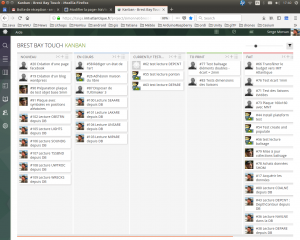
\includegraphics[width=14cm]{images/suiviProjet/kanban-300x240.png}
	}
	\begin{figure}[ht]
		\caption{\label{x3dRadeBrest}\textit{Un extrait du panneau KANBAN du projet}}
	\end{figure}
\end{center}
%%%%%%%%%%%%%%%%%%%%%%%%%%%%%%%%%%%%%%%%%%%%%%%%%%%%%%%%%%%%%%%%%
\section{Diff�rents types de cartes imprimables}
A partir d'une interface l'utilisateur peut choisir diff�rentes configurations de donn�es � visualiser.
\subsection{Mod�le num�rique de terrain + cartographie marine}
La partie terrestre est r�alis�e � partir des donn�es de l'IGN ou d'une autre source de telle que GeoTopo30 ou SRTM. La mer est une surface plane et un ensemble d'informations maritimes est extrait des cartes produites par le SHOM. 
%%%%%%%%%%%%%%%%%%%%%%%%%%%%%%%%%%%%%%%%%%%%%%%%%%%%%%%%%%%%%%%%%
\begin{center}
	\framebox[1\width]{
		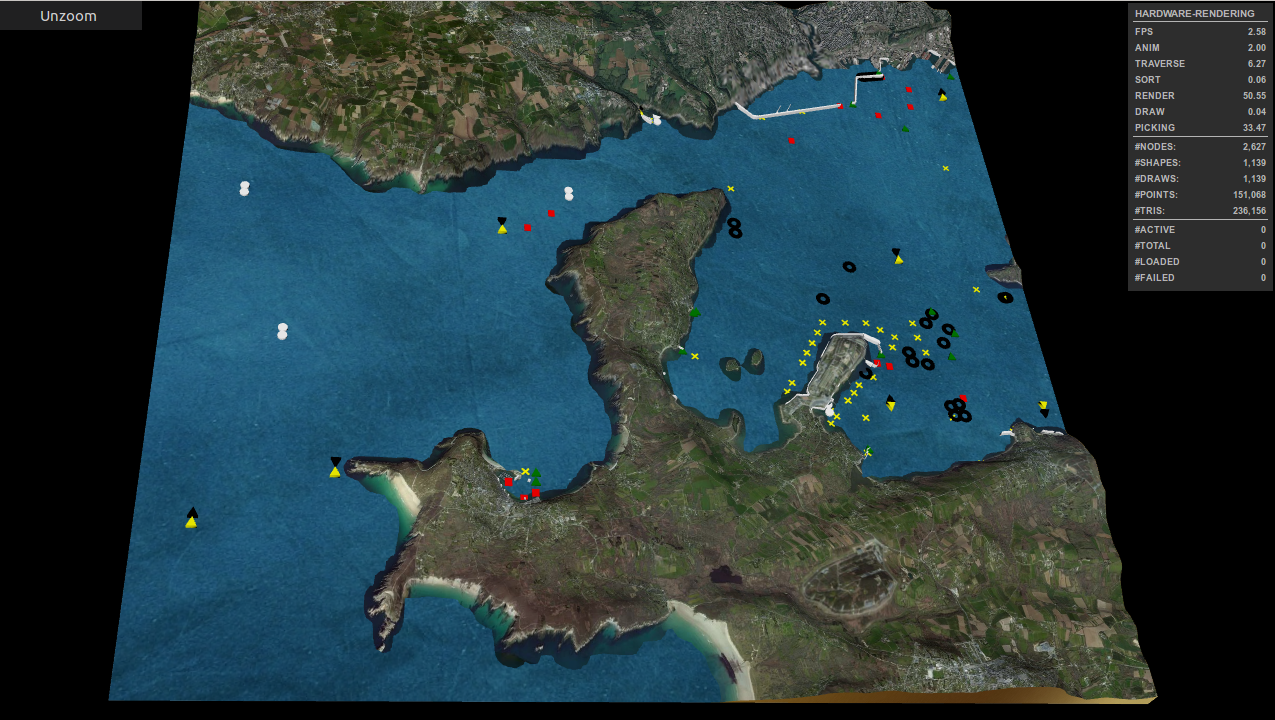
\includegraphics[width=14cm]{images/stl/x3dRade.png}
	}
	\begin{figure}[ht]
		\caption{\label{x3dRadeBrest}\textit{Rade de Brest }}
	\end{figure}
\end{center}
%%%%%%%%%%%%%%%%%%%%%%%%%%%%%%%%%%%%%%%%%%%%%%%%%%%%%%%%%%%%%%%%%
\subsection{Mod�le num�rique de terrain de la  bathym�trie}
%%%%%%%%%%%%%%%%%%%%%%%%%%%%%%%%%%%%%%%%%%%%%%%%%%%%%%%%%%%%%%%%%
\begin{center}
	\framebox[1\width]{
		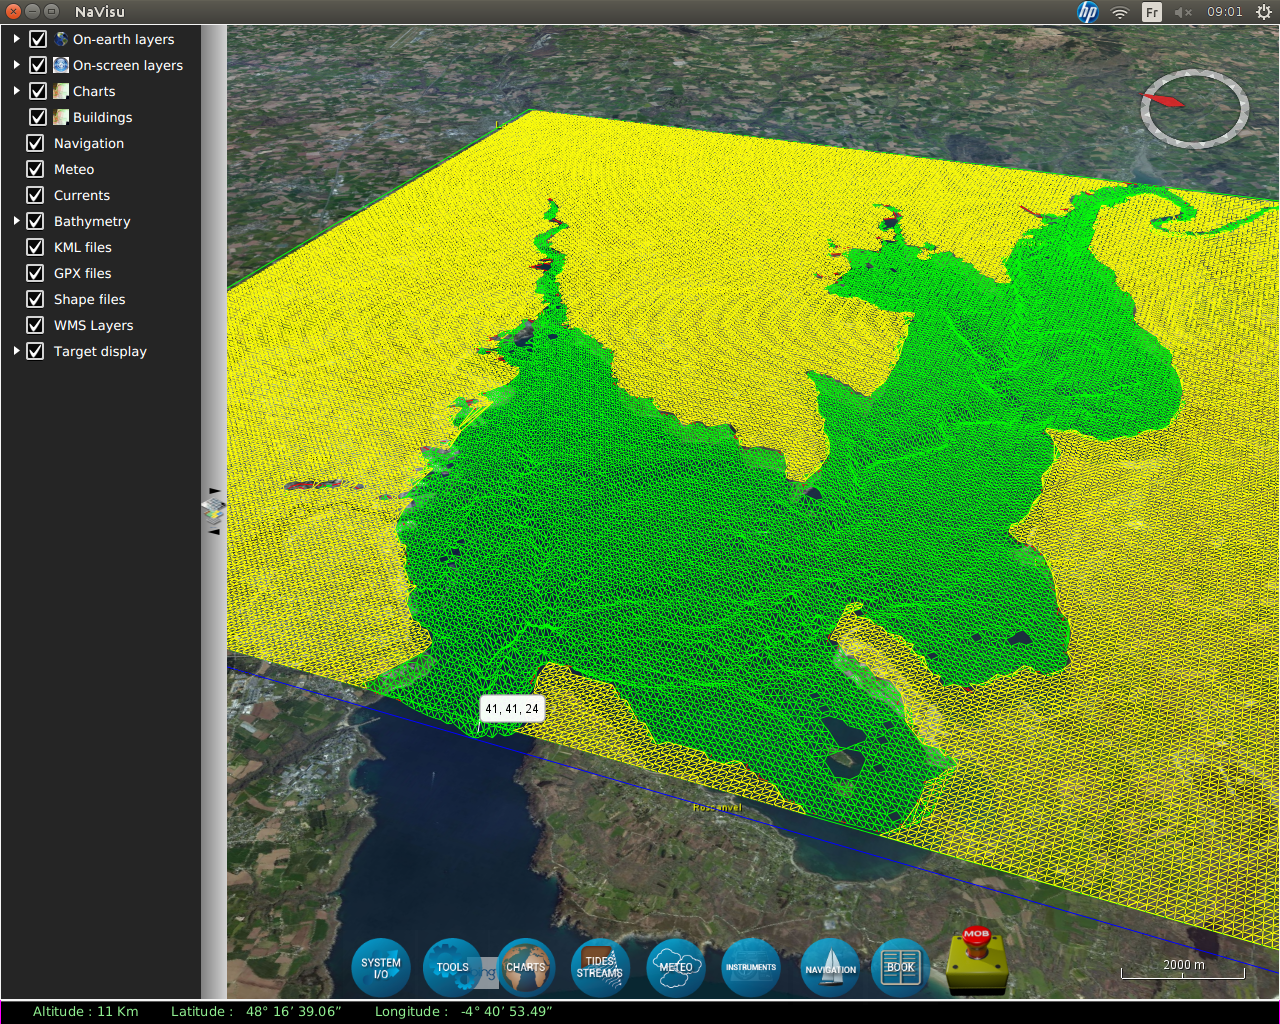
\includegraphics[width=14cm]{images/bathy/bathy_11.png}
	}
	\begin{figure}[ht]
		\caption{\label{MNTbathy}\textit{MNT bathym�trique }}
	\end{figure}
\end{center}
%%%%%%%%%%%%%%%%%%%%%%%%%%%%%%%%%%%%%%%%%%%%%%%%%%%%%%%%%%%%%%%%%
Afin d'offrir une connaissance des focnds marins, les donn�es bathym�triques araissent sous forme d'un mod�le num�rique de terrain. Le relief est alors plan.
\subsection{Mod�le num�rique de terrain altim�trique + mod�le num�rique de terrain bathym�trique}
Afin de donner une vision des fonds marins, dans cette configuration, pour la france,  on repr�sente les donn�es bathym�trique du SHOM sous forme d'un mod�le num�rique de terrain. Les donn�es altim�triques proviennent de l'IGN ou du SRTM, on proc�de alors � la fucion des donn�es.
%%%%%%%%%%%%%%%%%%%%%%%%%%%%%%%%%%%%%%%%%%%%%%%%%%%%%%%%%%%%%%%%%
\begin{center}
	\framebox[1\width]{
		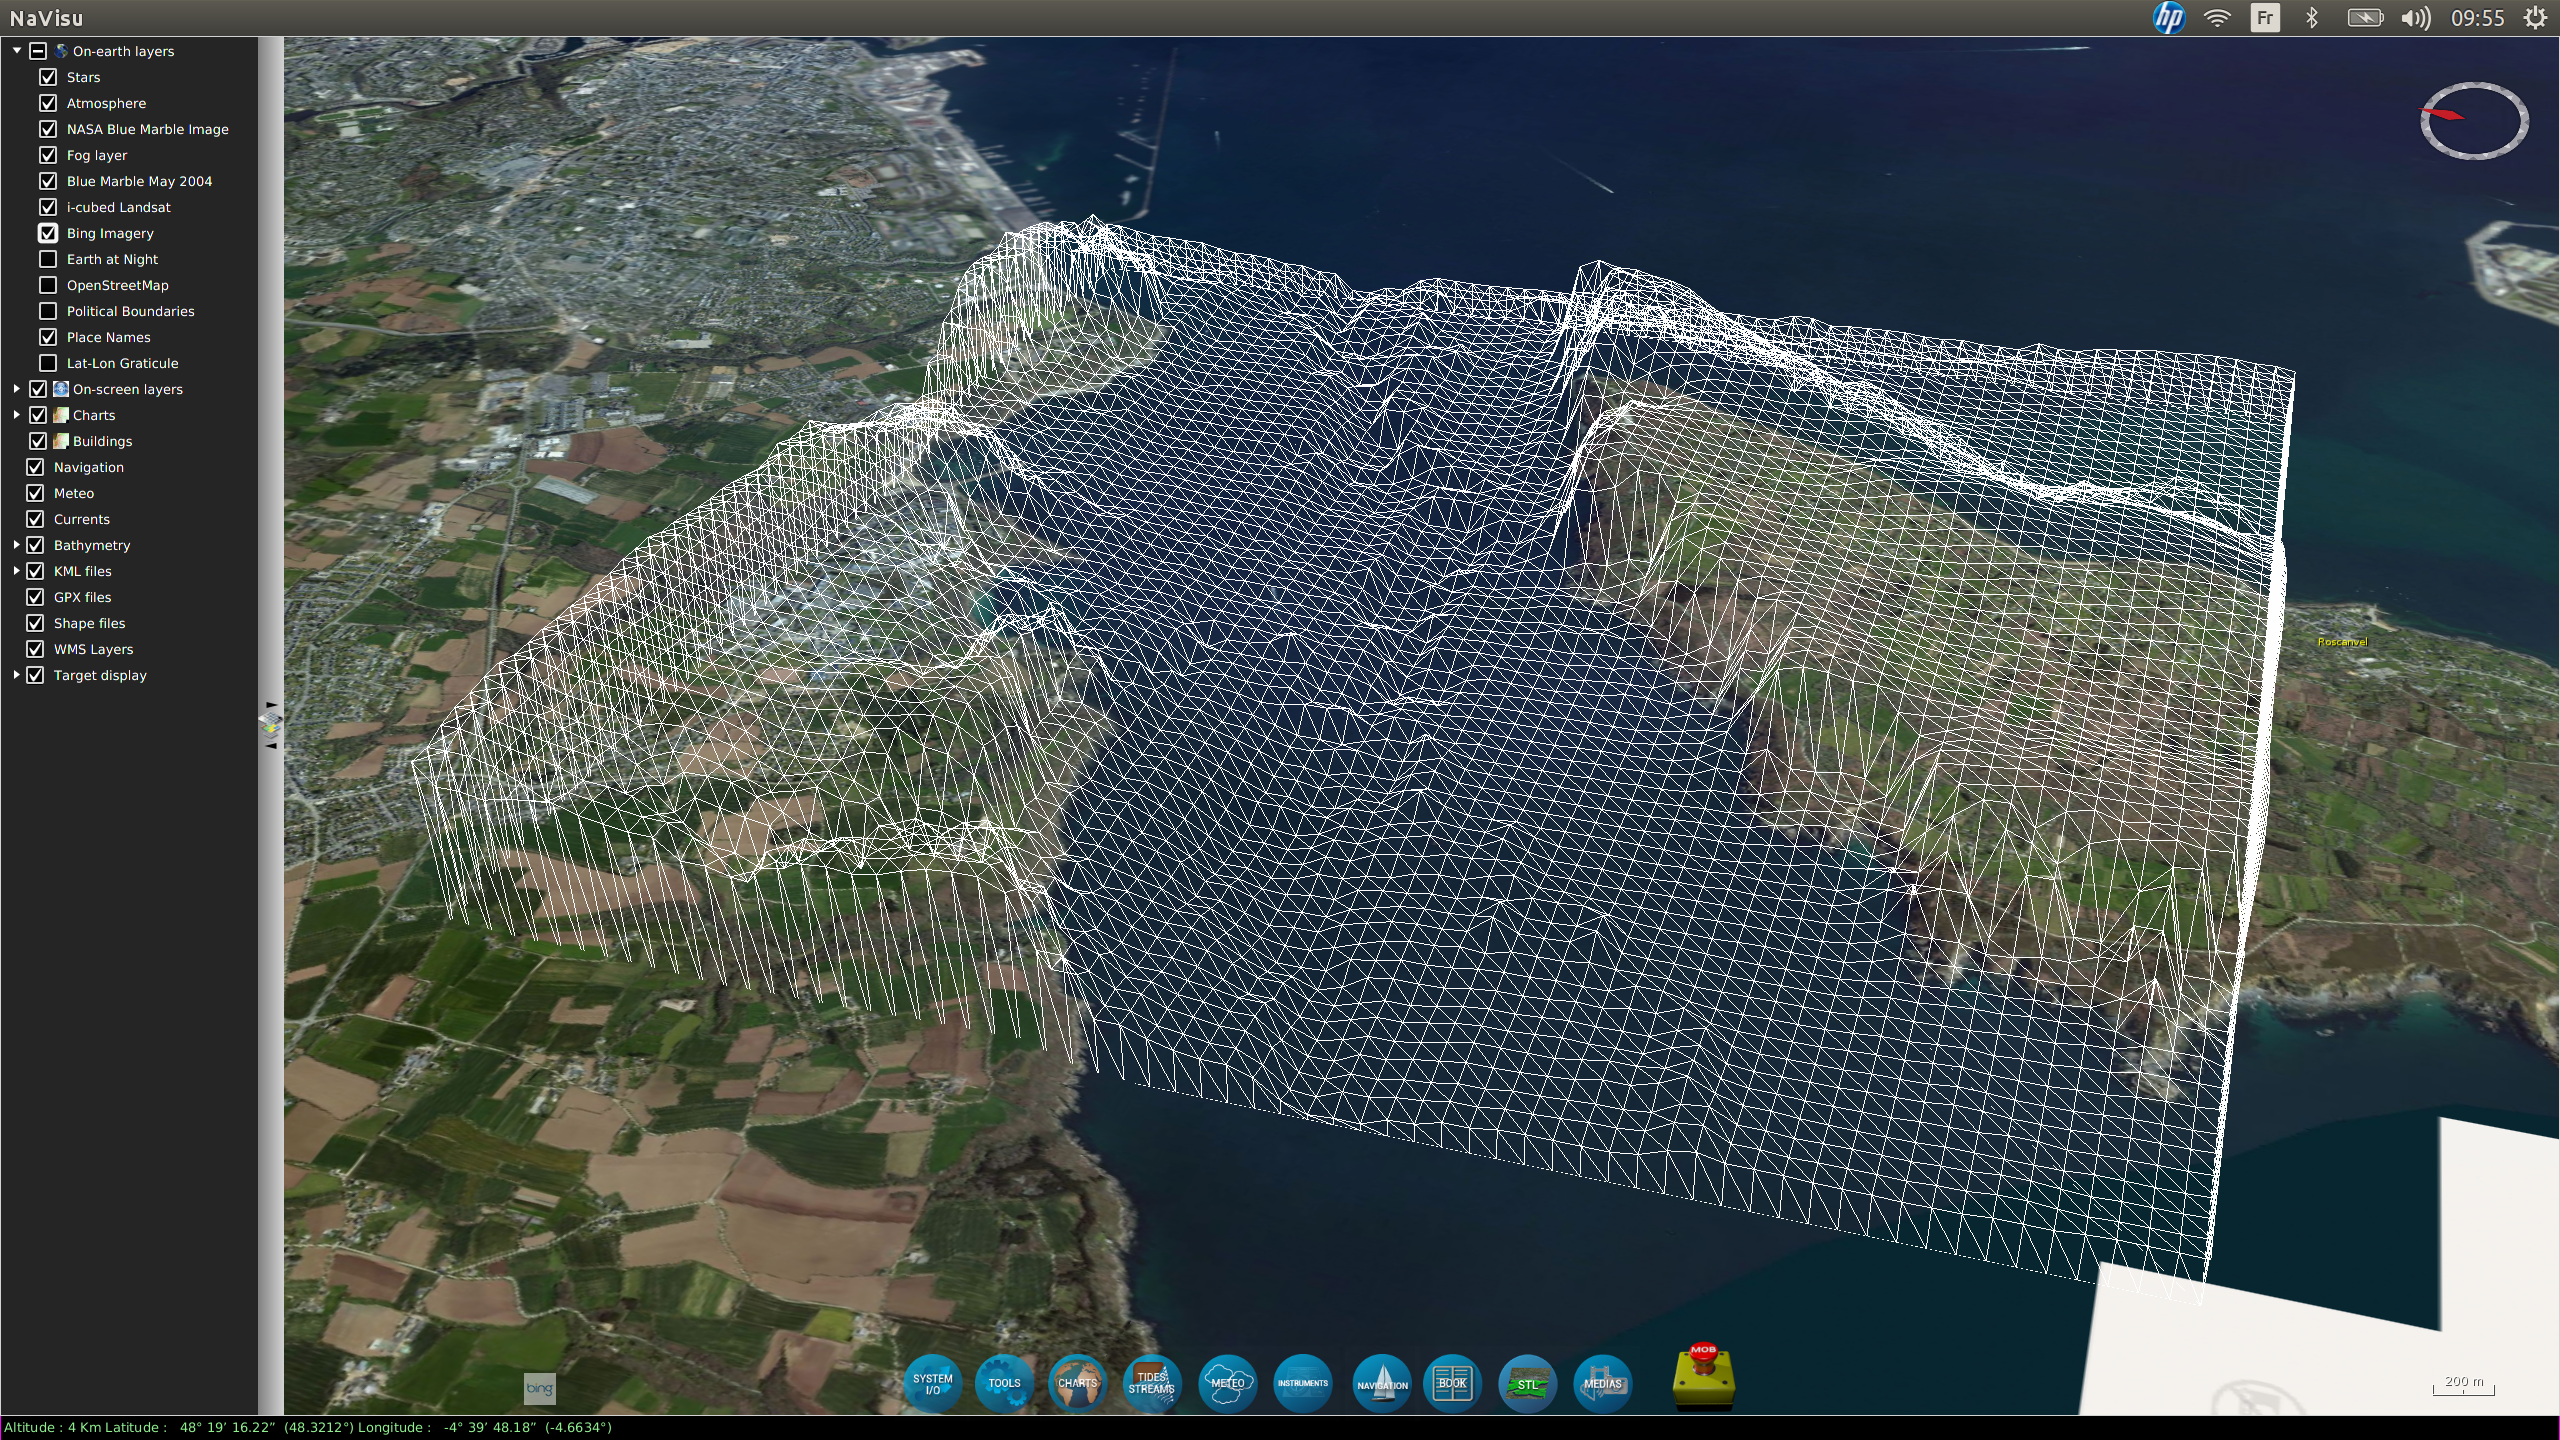
\includegraphics[width=14cm]{images/stl/mntAlti.png}
	}
	\begin{figure}[ht]
		\caption{\label{mntAlti}\textit{Les mod�les num�riques de terrain altim�trique et bathym�trique issus des donn�es IGN et SHOM}}
	\end{figure}
\end{center}
%%%%%%%%%%%%%%%%%%%%%%%%%%%%%%%%%%%%%%%%%%%%%%%%%%%%%%%%%%%%%%%%%

\subsection{Mod�le num�rique de terrain altim�trique + isobathym�triques}
Les isobathes sont issues de la cartographie vectorielle du SHOM ou de la NOAA.
%%%%%%%%%%%%%%%%%%%%%%%%%%%%%%%%%%%%%%%%%%%%%%%%%%%%%%%%%%%%%%%%%
\begin{center}
	\framebox[1\width]{
		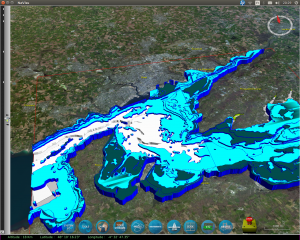
\includegraphics[width=14cm]{images/bathy/depare_4-300x240.png}
	}
	\begin{figure}[ht]
		\caption{\label{mntAlti}\textit{Les mod�les num�riques de terrain altim�trique et DepthArea de la cartographie du SHOM}}
	\end{figure}
\end{center}
%%%%%%%%%%%%%%%%%%%%%%%%%%%%%%%%%%%%%%%%%%%%%%%%%%%%%%%%%%%%%%%%%
%%%%%%%%%%%%%%%%%%%%%%%%%%%%%%%%%%%%%%%%%%%%%%%%%%%%%%%%%%%%%%%%%
\begin{center}
	\framebox[1\width]{
		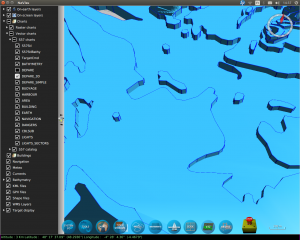
\includegraphics[width=14cm]{images/bathy/depareDBSimple3D-300x240.png}
	}
	\begin{figure}[ht]
		\caption{\label{mntAlti}\textit{Les mod�les num�riques de terrain altim�trique et DepthArea de la cartographie du SHOM}}
	\end{figure}
\end{center}
%%%%%%%%%%%%%%%%%%%%%%%%%%%%%%%%%%%%%%%%%%%%%%%%%%%%%%%%%%%%%%%%%

\subsection{Mod�le num�rique de terrain + cartographie marine + bathym�trie}
Ici aussi la bathym�trie est repr�sent�e sous forme "d'escaliers" correspondant aux isobathes des cartes marines. Il est aussi possible de rajouter les information maritimes : bou�es, phares, \ldots
\section{Tests}
%%%%%%%%%%%%%%%%%%%%%%%%%%%%%%%%%%%%%%%%%%%%%%%%%%%%%%%%%%%%%%%%%
\begin{center}
	\framebox[1\width]{
		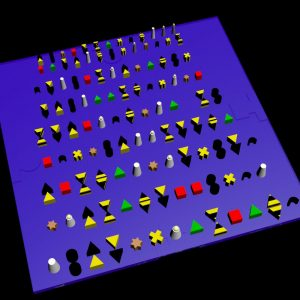
\includegraphics[width=14cm]{images/tests/all-300x300.jpg}
	}
	\begin{figure}[ht]
		\caption{\label{mntAlti}\textit{Recherche de la bonne repr�sentation du balisage : planche g�n�rale}}
	\end{figure}
\end{center}
%%%%%%%%%%%%%%%%%%%%%%%%%%%%%%%%%%%%%%%%%%%%%%%%%%%%%%%%%%%%%%%%%
%%%%%%%%%%%%%%%%%%%%%%%%%%%%%%%%%%%%%%%%%%%%%%%%%%%%%%%%%%%%%%%%%
\begin{center}
	\framebox[1\width]{
		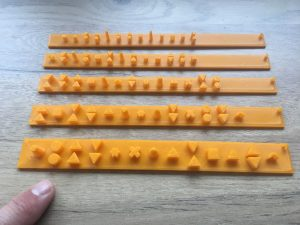
\includegraphics[width=14cm]{images/tests/lines34567-300x225.jpg}
	}
	\begin{figure}[ht]
		\caption{\label{mntAlti}\textit{Recherche de la bonne repr�sentation du balisage}}
	\end{figure}
\end{center}
%%%%%%%%%%%%%%%%%%%%%%%%%%%%%%%%%%%%%%%%%%%%%%%%%%%%%%%%%%%%%%%%%
%%%%%%%%%%%%%%%%%%%%%%%%%%%%%%%%%%%%%%%%%%%%%%%%%%%%%%%%%%%%%%%%%
\begin{center}
	\framebox[1\width]{
		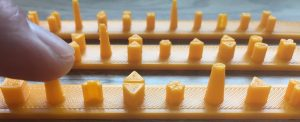
\includegraphics[width=14cm]{images/tests/lines2_3mm_et_1_4mmet5mm-300x122.jpg}
	}
	\begin{figure}[ht]
		\caption{\label{mntAlti}\textit{Recherche de la bonne repr�sentation du balisage}}
	\end{figure}
\end{center}
%%%%%%%%%%%%%%%%%%%%%%%%%%%%%%%%%%%%%%%%%%%%%%%%%%%%%%%%%%%%%%%%%
%%%%%%%%%%%%%%%%%%%%%%%%%%%%%%%%%%%%%%%%%%%%%%%%%%%%%%%%%%%%%%%%%
\chapter{Les contraintes}
%%%%%%%%%%%%%%%%%%%%%%%%%%%%%%%%%%%%%%%%%%%%%%%%%%%%%%%%%%%%%%%%%

\section{Contraintes technologiques}

\subsection{Le tuilage}
Les imprimantes 3D dont dispose l'utilisateur peuvent ne pas correspondre aux dimensions que l'on souhaite avoir pour les cartes. Dans ce cas nous proposons un tuilage, qui consiste � d�couper la zone d�finie en une s�rie de petites zones. Les cartes imprim�es seront ensuite reli�es par aimantation. A l'heure actuelle, � cause des contraintes sur les imprimantes ces tuiles sont carr�es.
\section{Contraintes g�od�siques}
\subsection{Syst�mes de coordonn�es}
Les donn�es maritimes mondiales sont g�n�ralement fournies dans le r�f�rentiel WGS 84 (EPSG:4326), en France les dnn�es altim�triques distribu�es par l'IGN ou les donn�es LIDAR de la cote sont dans le r�f�rentiel REF 93 avec la projection  Lambert93. Pour effectuer la fusionn des donn�es il convient de proc�der au changement de projection.
%%%%%%%%%%%%%%%%%%%%%%%%%%%%%%%%%%%%%%%%%%%%%%%%%%%%%%%%%%%%%%%%%%%%%%%
\begin{center}
	\framebox[1\width]{
		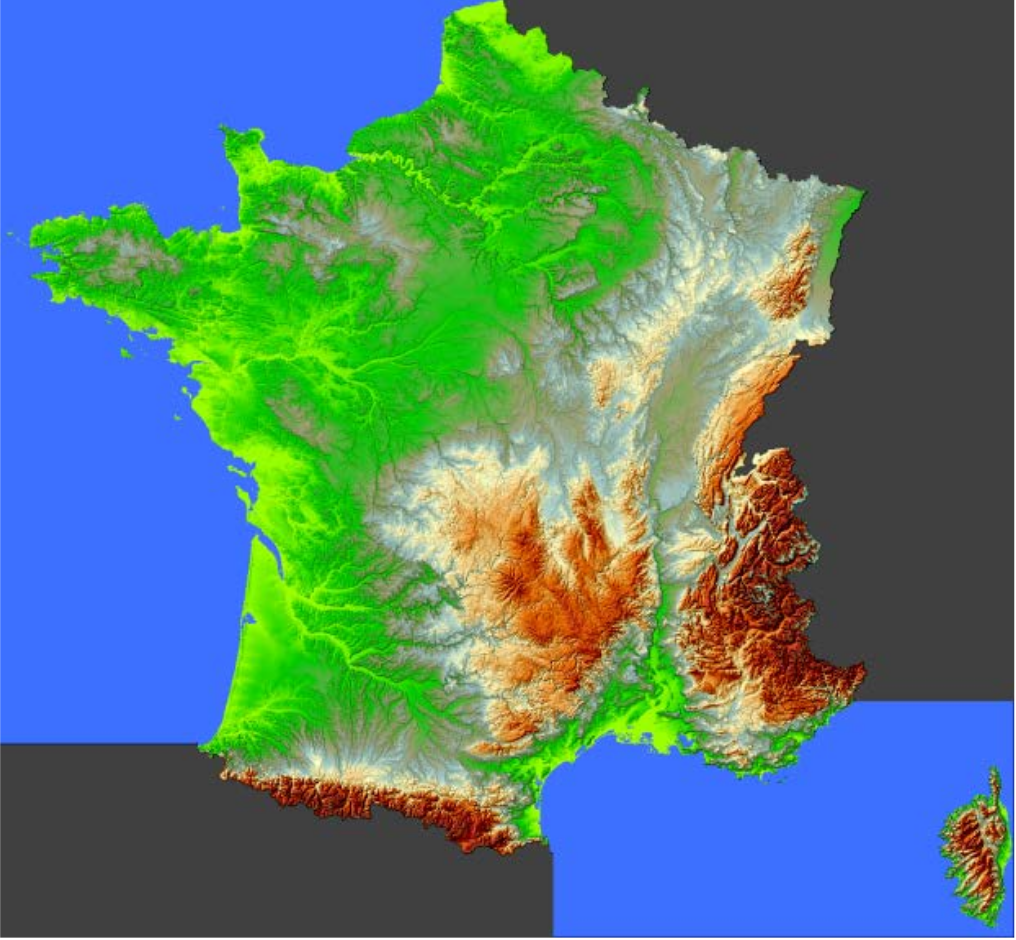
\includegraphics[width=16cm]{images/dem/ign1.png}
	}
	\begin{figure}[ht]
		\caption{\label{bathyDB}\textit{Repr�sentation hypsom�trique du relief m�tropolitain}}
	\end{figure}
\end{center}
%%%%%%%%%%%%%%%%%%%%%%%%%%%%%%%%%%%%%%%%%%%%%%%%%%%%%%%%%%%%%%%%%
\section{Contraintes s�miologique}
C'est l'objet de notre partenaire l'association Orion.
Il s'agit d'maginer et reconstruire un ensemble de symboles cartographiques pour les non voyants
%%%%%%%%%%%%%%%%%%%%%%%%%%%%%%%%%%%%%%%%%%%%%%%%%%%%%%%%%%%%%%%%%
\chapter{Les sources de donn�es}
%%%%%%%%%%%%%%%%%%%%%%%%%%%%%%%%%%%%%%%%%%%%%%%%%%%%%%%%%%%%%%%%%

\section{Altim�trie}
\subsection{Sources}
\begin{itemize}
\item Space Shuttle Radar Topography Mission (SRTM)
%%%%%%%%%%%%%%%%%%%%%%%%%%%%%%%%%%%%%%%%%%%%%%%%%%%%%%%%%%%%%%%%%%%%%%
\begin{center}
	\framebox[1\width]{
		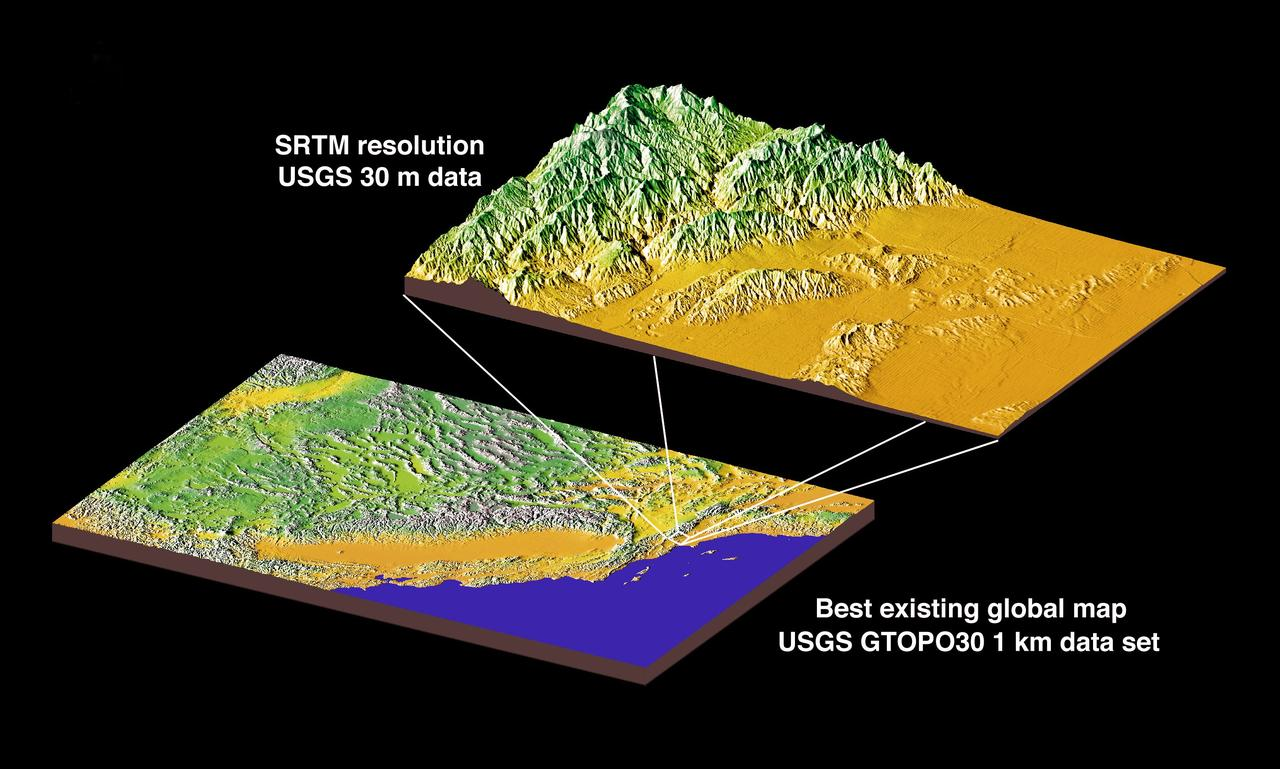
\includegraphics[width=16cm]{images/dem/srtm.jpg}
	}
	\begin{figure}[ht]
		\caption{\label{ignDB}\textit{Space Shuttle Radar Topography Mission (SRTM)}}
	\end{figure}
\end{center}
%%%%%%%%%%%%%%%%%%%%%%%%%%%%%%%%%%%%%%%%%%%%%%%%%%%%%%%%%%%%%%%%%%%%%%%

\item L'IGN
\\
Actuellement (2018)  l'IGN :
\href{http://professionnels.ign.fr/bdalti}{BD ALTI}, fichiers : {\tt BDALTIV2\_75M\_FXX\_xxxx\_xxxx\_MNT\_LAMB93\_IGN69.asc}, fourni gracieusement des donn�es altim�triques tous les 75m. Nous pouvons utiliser ces donn�es � partir de nos bases de donn�es, mais nous pr�f�rons les donn�es du SRTM, tous les 30m, depuis 2014. Le travail effectu� pour d�codage des donn�es de l'IGN, ainsi que la reprojection vers le syst�me EPSG : 4326, nous sera utile pour l'utilisation des donn�es LIDAR.
\subsection{Mise en \oe uvre}
La distribution des donn�es de l'IGN, vient sous forme d'une collection de fichiers au format .asc. Chaque fichier repr�sente 75Km$�$ sur la terre, � raison d'un point tous les 75m, ils sont donc relativement volumineux. 
%%%%%%%%%%%%%%%%%%%%%%%%%%%%%%%%%%%%%%%%%%%%%%%%%%%%%%%%%%%%%%%%%%%%%%
\begin{center}
	\framebox[1\width]{
		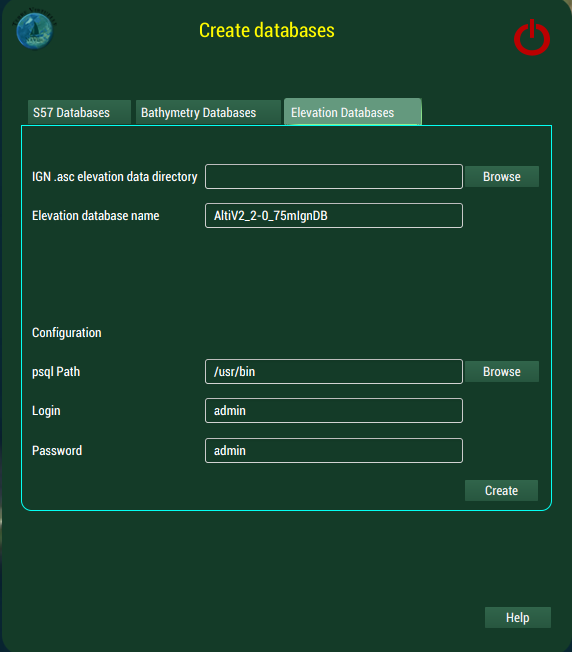
\includegraphics[width=16cm]{images/utilisation/altiDB.png}
	}
	\begin{figure}[ht]
		\caption{\label{ignDB}\textit{Chargement des donn�es dans la base BD ALTI}}
	\end{figure}
\end{center}
%%%%%%%%%%%%%%%%%%%%%%%%%%%%%%%%%%%%%%%%%%%%%%%%%%%%%%%%%%%%%%%%%%%%%%%
\subsection{Etendue spatiale}
%%%%%%%%%%%%%%%%%%%%%%%%%%%%%%%%%%%%%%%%%%%%%%%%%%%%%%%%%%%%%%%%%%%%%%
\begin{center}
	\framebox[1\width]{
		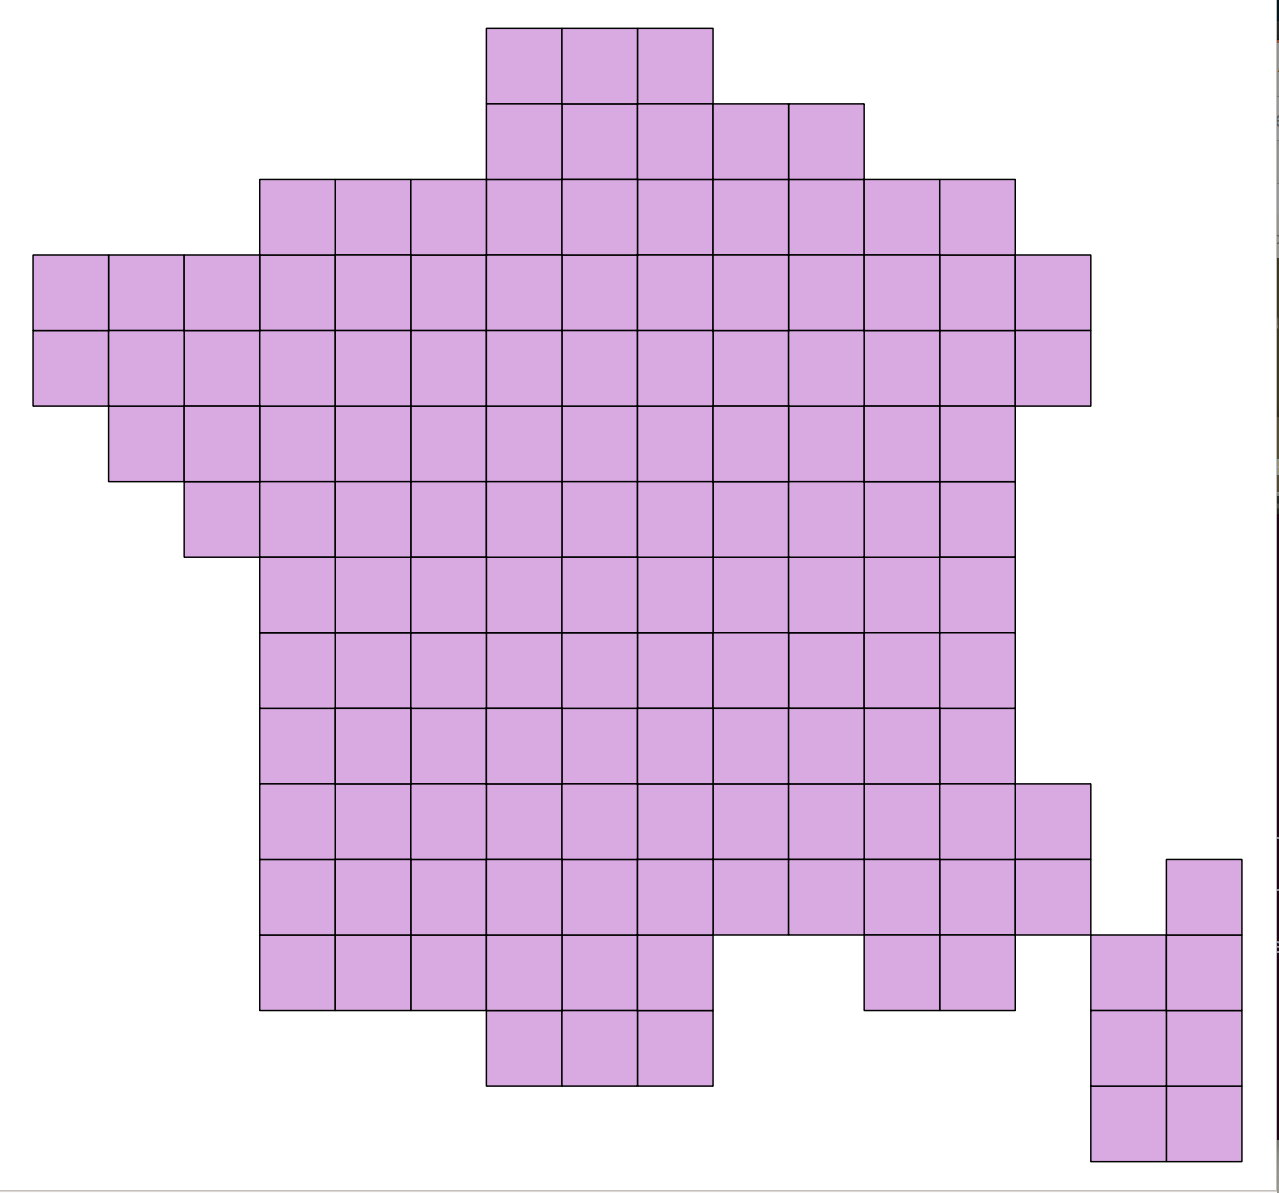
\includegraphics[width=16cm]{images/dem/ign.png}
	}
	\begin{figure}[ht]
		\caption{\label{ignDB}\textit{Etendue du projet BD ALTI}}
	\end{figure}
\end{center}
%%%%%%%%%%%%%%%%%%%%%%%%%%%%%%%%%%%%%%%%%%%%%%%%%%%%%%%%%%%%%%%%%%%%%%%
\end{itemize}
\section{Bathym�trie}
\subsection{Sources}
%%%%%%%%%%%%%%%%%%%%%%%%%%%%%%%%%%%%%%%%%%%%%%%%%%%%%%%%%%%%%%%%%%%%%%
\begin{center}
	\framebox[1\width]{
		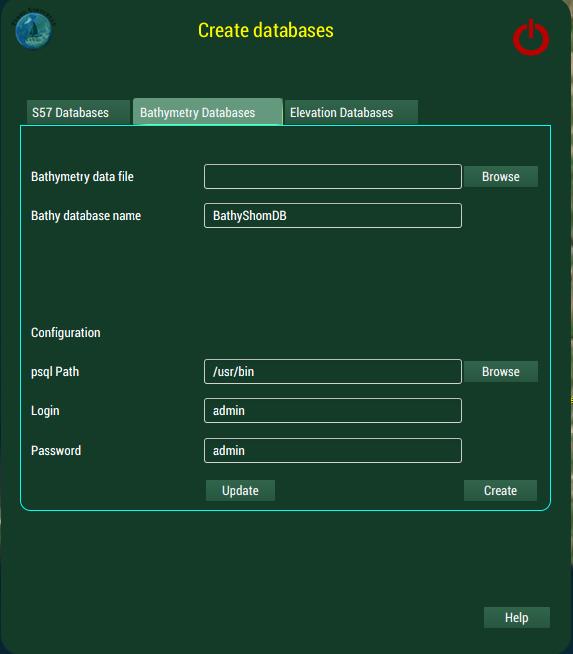
\includegraphics[width=16cm]{images/utilisation/bathyDB.png}
	}
	\begin{figure}[ht]
		\caption{\label{ignDB}\textit{Chargement des donn�es dans la base BD BATHY}}
	\end{figure}
\end{center}
%%%%%%%%%%%%%%%%%%%%%%%%%%%%%%%%%%%%%%%%%%%%%%%%%%%%%%%%%%%%%%%%%%%%%%%
\subsection{Etendue spatiale}
%%%%%%%%%%%%%%%%%%%%%%%%%%%%%%%%%%%%%%%%%%%%%%%%%%%%%%%%%%%%%%%%%%%%%%%
\begin{center}
	\framebox[1\width]{
		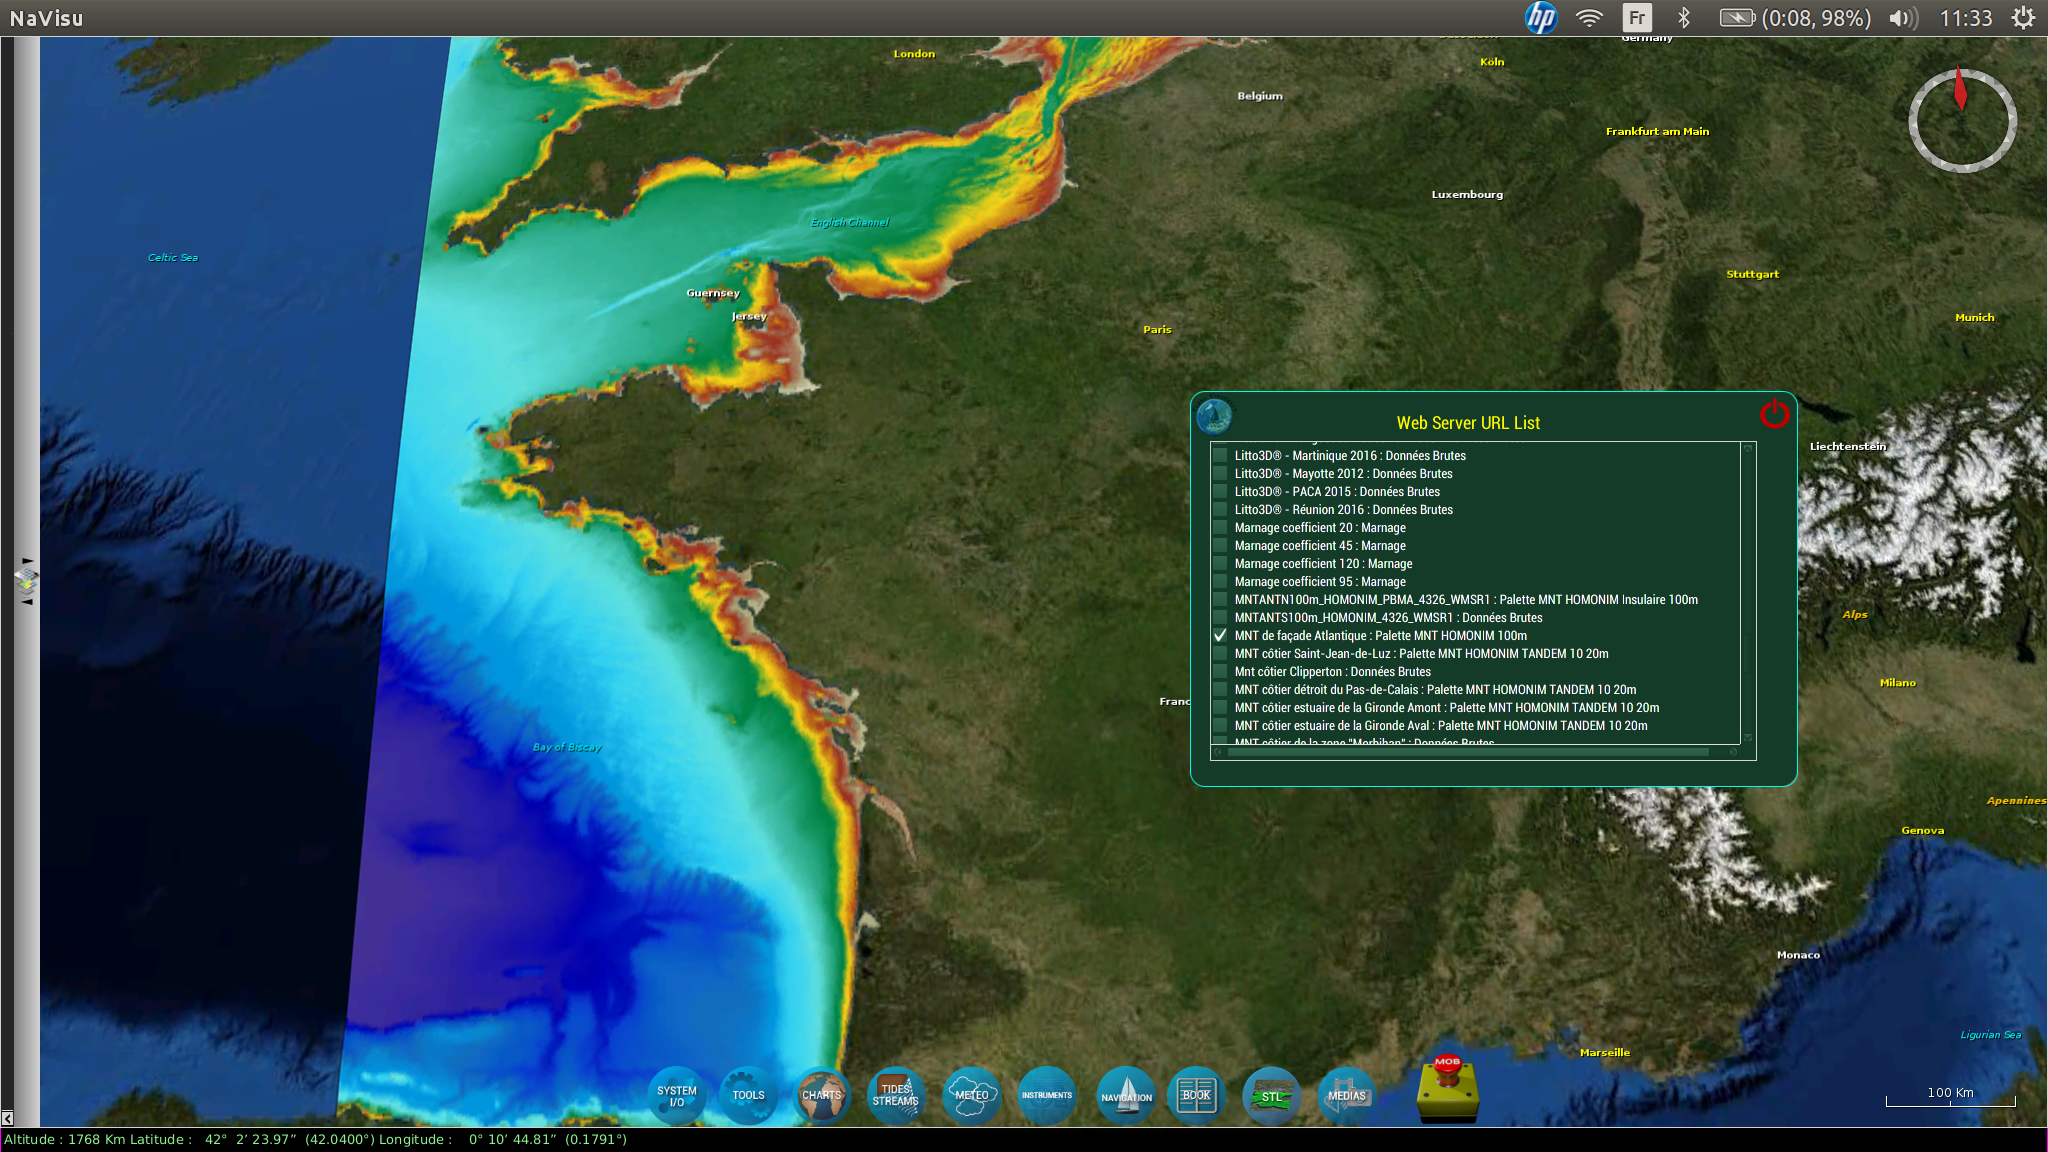
\includegraphics[width=16cm]{images/bathy/homonim_0.png}
	}
	\begin{figure}[ht]
		\caption{\label{bathyDB}\textit{Etendue du projet Homonim PBMA}}
	\end{figure}
\end{center}
%%%%%%%%%%%%%%%%%%%%%%%%%%%%%%%%%%%%%%%%%%%%%%%%%%%%%%%%%%%%%%%%%

%%%%%%%%%%%%%%%%%%%%%%%%%%%%%%%%%%%%%%%%%%%%%%%%%%%%%%%%%%%%%%%%%
\begin{center}
	\framebox[1\width]{
		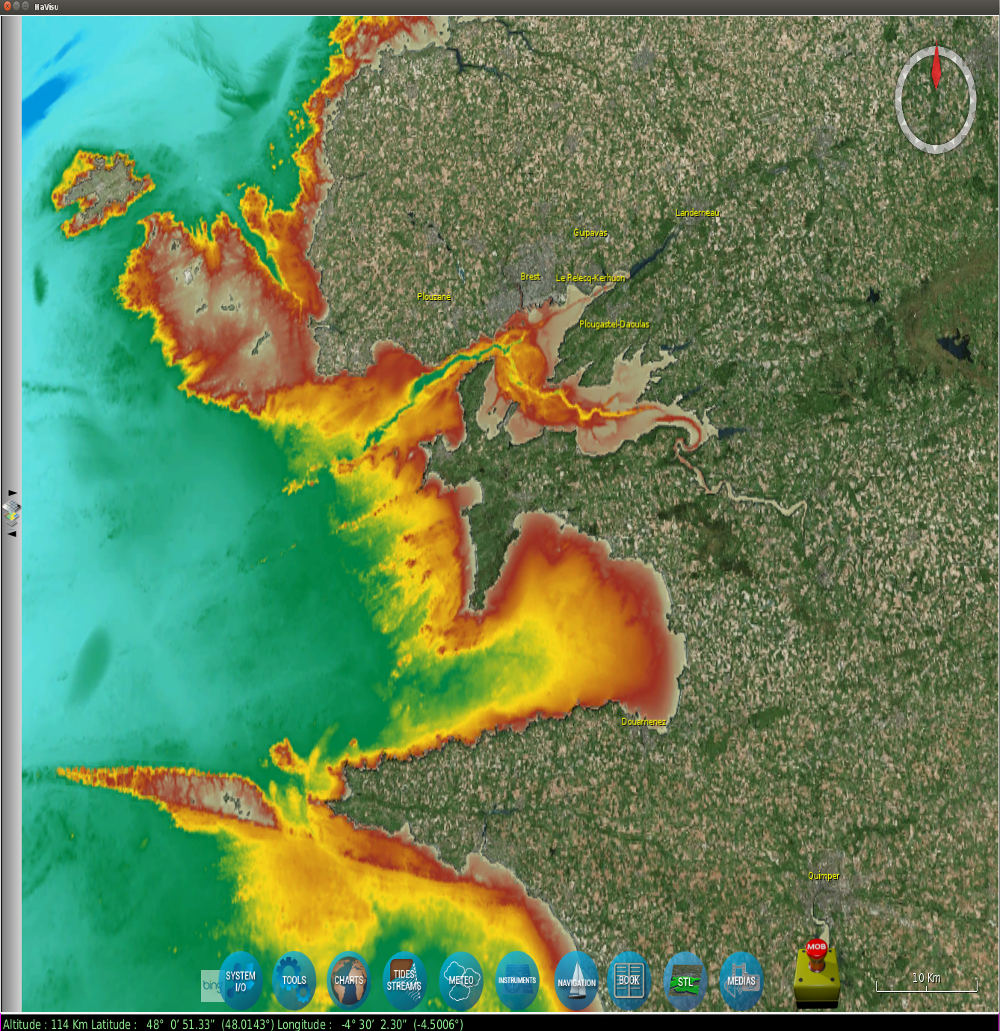
\includegraphics[width=15cm]{images/bathy/homonim.png}
	}
	\begin{figure}[ht]
		\caption{\label{bathyDB}\textit{MNT bathym�trique de la fa�ade Atlantique � une r�solution de 0.001�(~111m)}}
	\end{figure}
	
\end{center}
%%%%%%%%%%%%%%%%%%%%%%%%%%%%%%%%%%%%%%%%%%%%%%%%%%%%%%%%%%%%%%%%
\subsection{Mise en \oe uvre}

\section{Cartographie}
\subsection{Sources}
SHOM
NOAA
%%%%%%%%%%%%%%%%%%%%%%%%%%%%%%%%%%%%%%%%%%%%%%%%%%%%%%%%%%%%%%%%%%%%%%
\begin{center}
	\framebox[1\width]{
		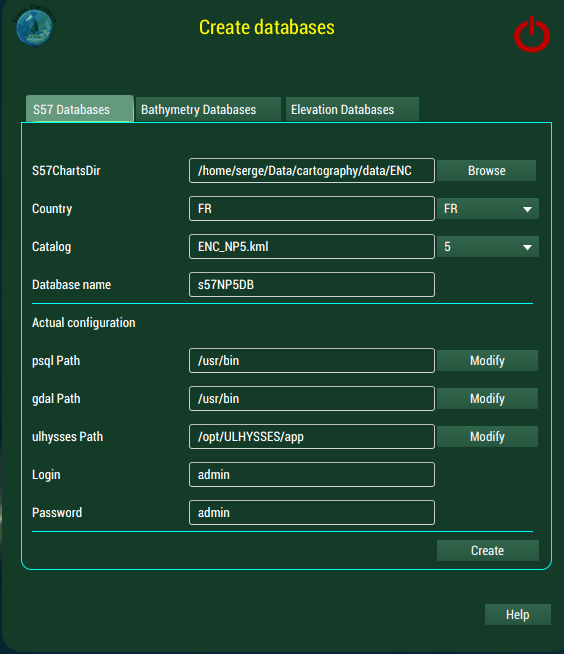
\includegraphics[width=16cm]{images/utilisation/s57DB.png}
	}
	\begin{figure}[ht]
		\caption{\label{ignDB}\textit{Chargement des donn�es dans une des bases cartographiques S57}}
	\end{figure}
\end{center}
%%%%%%%%%%%%%%%%%%%%%%%%%%%%%%%%%%%%%%%%%%%%%%%%%%%%%%%%%%%%%%%%%%%%%%%
\subsection{Etendue spatiale}
\subsection{Mise en \oe uvre}



\section{Objets 3D g�or�f�renc�s}
\subsection{Sources}
\subsection{Mise en \oe uvre}
%%%%%%%%%%%%%%%%%%%%%%%%%%%%%%%%%%%%%%%%%%%%%%%%%%%%%%%%%%%%%%%%%
\begin{center}
	\framebox[1\width]{
		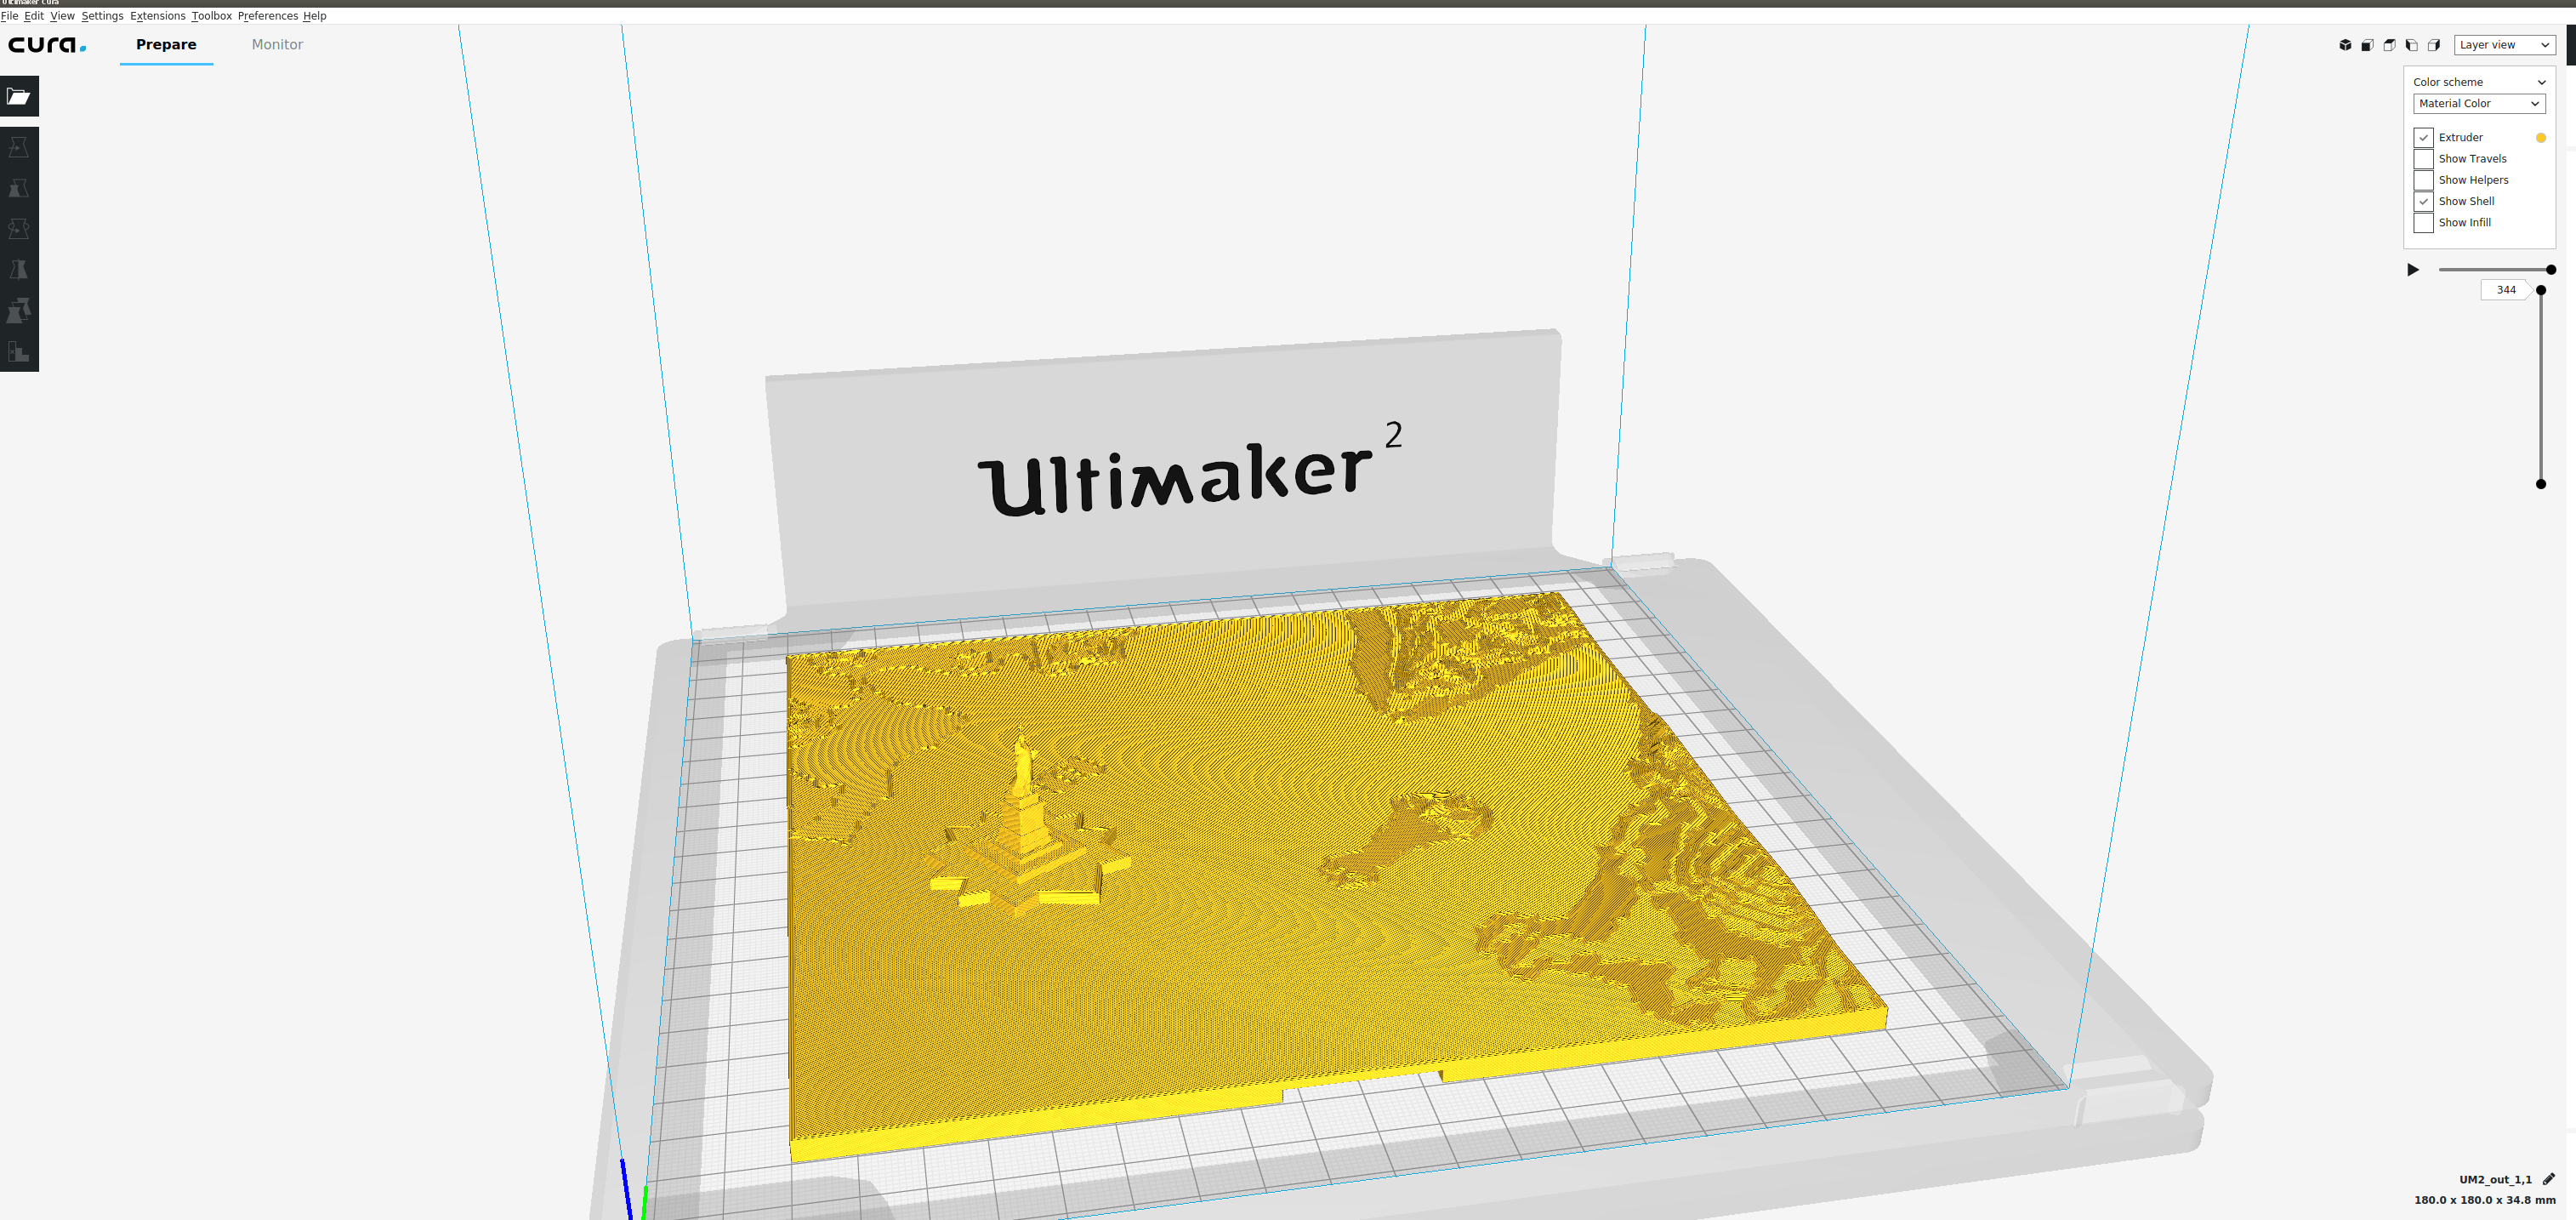
\includegraphics[width=14cm]{images/dae/nySTL.png}
	}
	\begin{figure}[ht]
		\caption{\label{MNTbathy}\textit{Entr�e de new York City }}
	\end{figure}
\end{center}
%%%%%%%%%%%%%%%%%%%%%%%%%%%%%%%%%%%%%%%%%%%%%%%%%%%%%%%%%%%%%%%%%

%%%%%%%%%%%%%%%%%%%%%%%%%%%%%%%%%%%%%%%%%%%%%%%%%%%%%%%%%%%%%%%%%
\chapter{L'export des donn�es}
%%%%%%%%%%%%%%%%%%%%%%%%%%%%%%%%%%%%%%%%%%%%%%%%%%%%%%%%%%%%%%%%%
\section{Export STL}
Le format STL (Standard Tessellation Language), initialement d�velopp� par {\bf 3D Systems}, est extr�mement simple. Un fichier STL d�crit les surfaces de mailles telles des caract�ristiques g�om�triques. Un solide est compos� de faces triangulaires, qui sont elles-m�mes compos�es d'une normale et de 3 sommets d�crits par leurs coordonn�es. 
\begin{center}
\begin{minipage}{12cm}
\begin{verbatim}
solid
  facet normal 0.0 -0.9882392306514677 0.15291573823970914 
    outer loop 
      vertex 137.95979903830215 138.60046315913647 4.0 
      vertex 137.57078026018425 136.08637518871737 4.807470290632069 
      vertex 137.95979903830215 138.60046315913647 4.807470290632069 
    endloop 
  endfacet 
  facet normal 0.0 -0.9882392306514677 0.15291573823970914 
    outer loop 
      vertex 137.95979903830215 138.60046315913647 4.0 
      vertex 137.57078026018425 136.08637518871737 4.0 
      vertex 137.57078026018425 136.08637518871737 4.807470290632069 
    endloop 
    endfacet 
end solid
\end{verbatim}
\end{minipage}
\end{center}
Ce format a l'avantage d'�tre accept� par la plupart des imprimantes, mais oblige le concepteur � faire de nombreux calculs. De plus la couleur n'est nativement pas support�e.
\section{Export 3MF}
\section{Export KML}
%%%%%%%%%%%%%%%%%%%%%%%%%%%%%%%%%%%%%%%%%%%%%%%%%%%%%%%%%%%%%%%%%
\begin{center}
	\framebox[1\width]{
		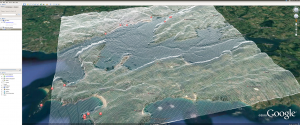
\includegraphics[width=15cm]{images/export/bathyshomaltiign-300x125.png}
	}
	\begin{figure}[ht]
		\caption{\label{kml}\textit{Export des donn�es en KML, visualisation sur Google Earth}}
	\end{figure}
\end{center}
%%%%%%%%%%%%%%%%%%%%%%%%%%%%%%%%%%%%%%%%%%%%%%%%%%%%%%%%%%%%%%%%%
%%%%%%%%%%%%%%%%%%%%%%%%%%%%%%%%%%%%%%%%%%%%%%%%%%%%%%%%%%%%%%%%%
\begin{center}
	\framebox[1\width]{
		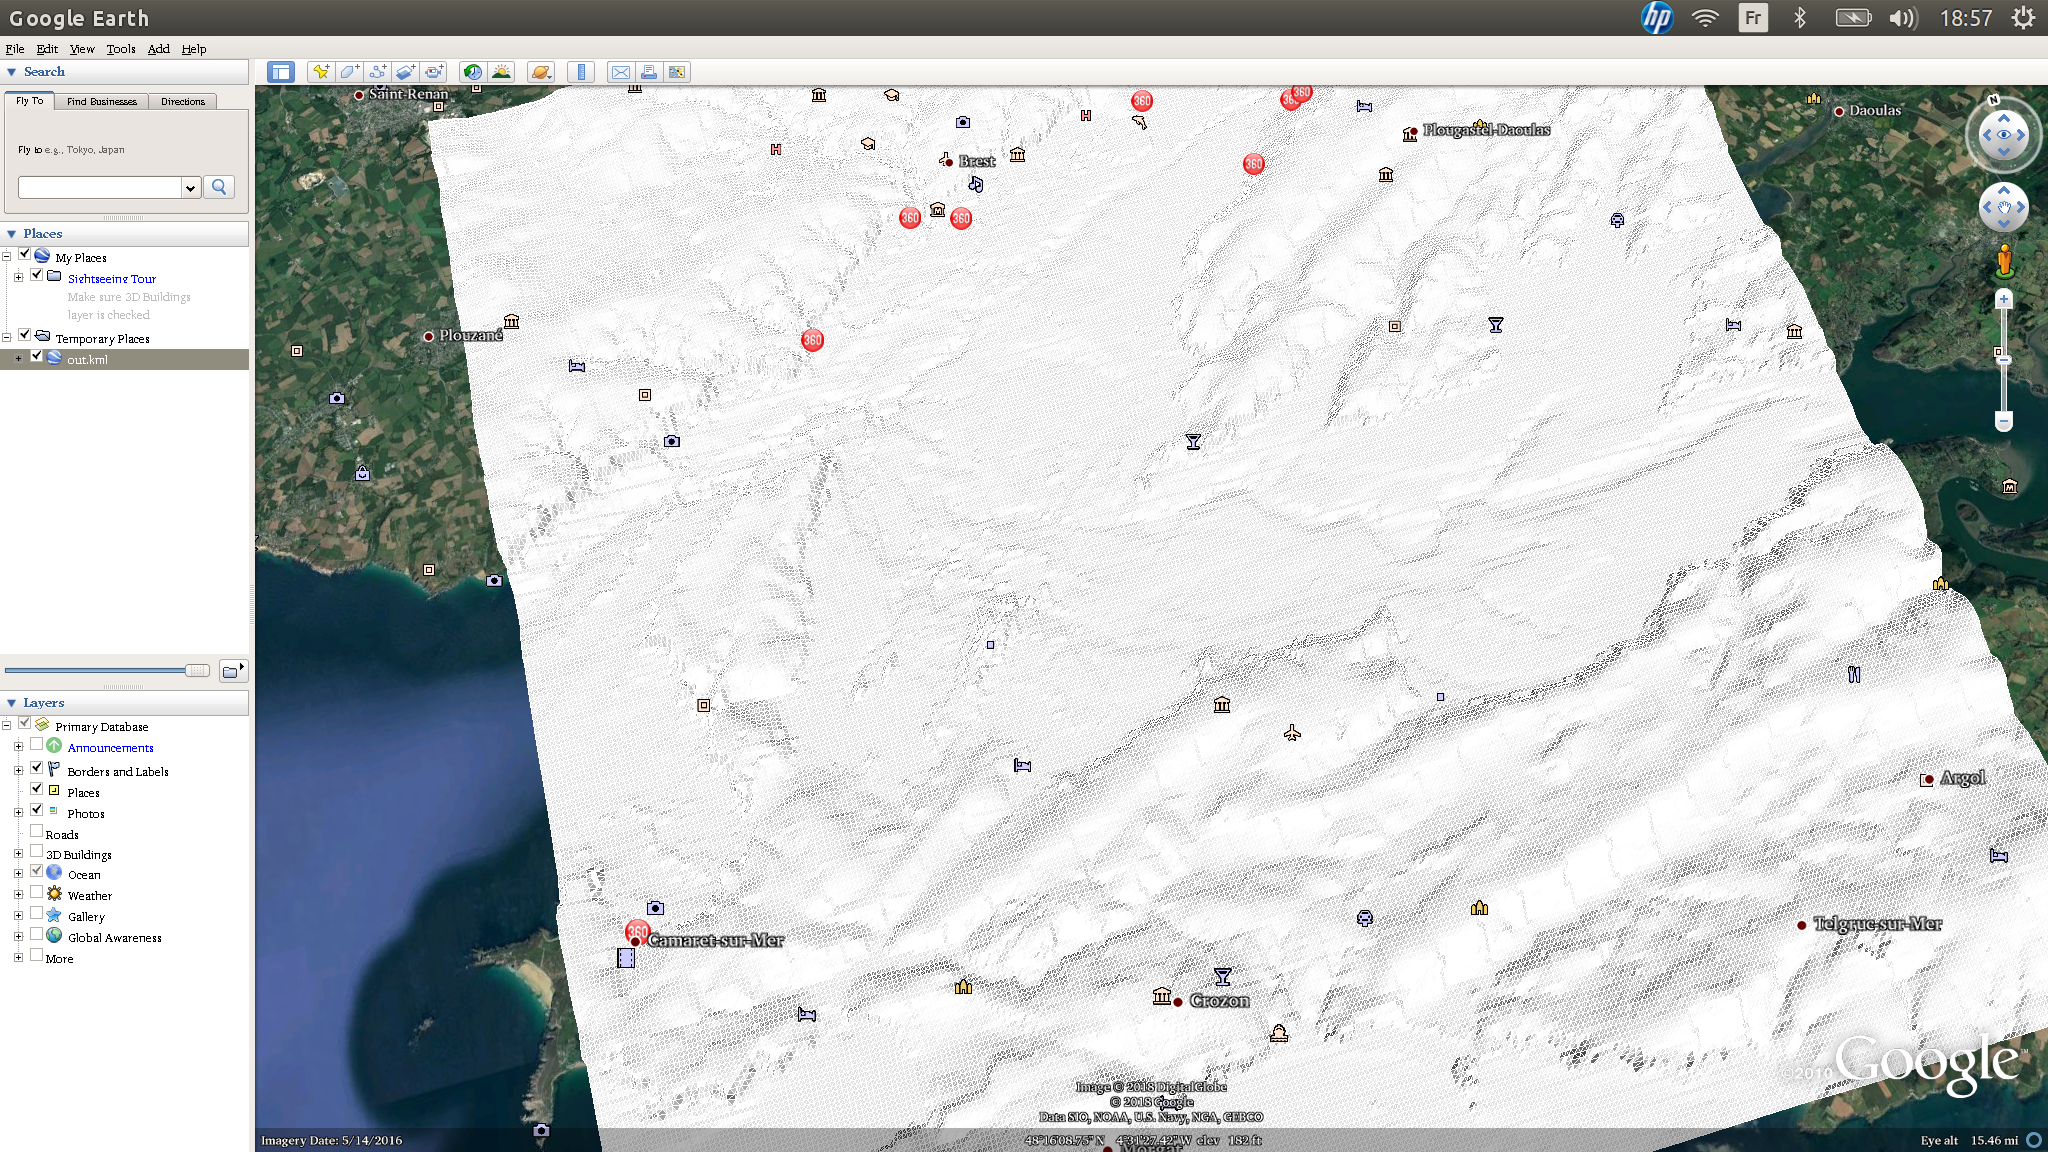
\includegraphics[width=15cm]{images/stl/kml.png}
	}
	\begin{figure}[ht]
		\caption{\label{kml}\textit{Export des donn�es en KML, visualisation en polygones sur Google Earth}}
	\end{figure}
\end{center}
%%%%%%%%%%%%%%%%%%%%%%%%%%%%%%%%%%%%%%%%%%%%%%%%%%%%%%%%%%%%%%%%%

\section{Export GeoTiff}
%%%%%%%%%%%%%%%%%%%%%%%%%%%%%%%%%%%%%%%%%%%%%%%%%%%%%%%%%%%%%%%%%
\begin{center}
	\framebox[1\width]{
		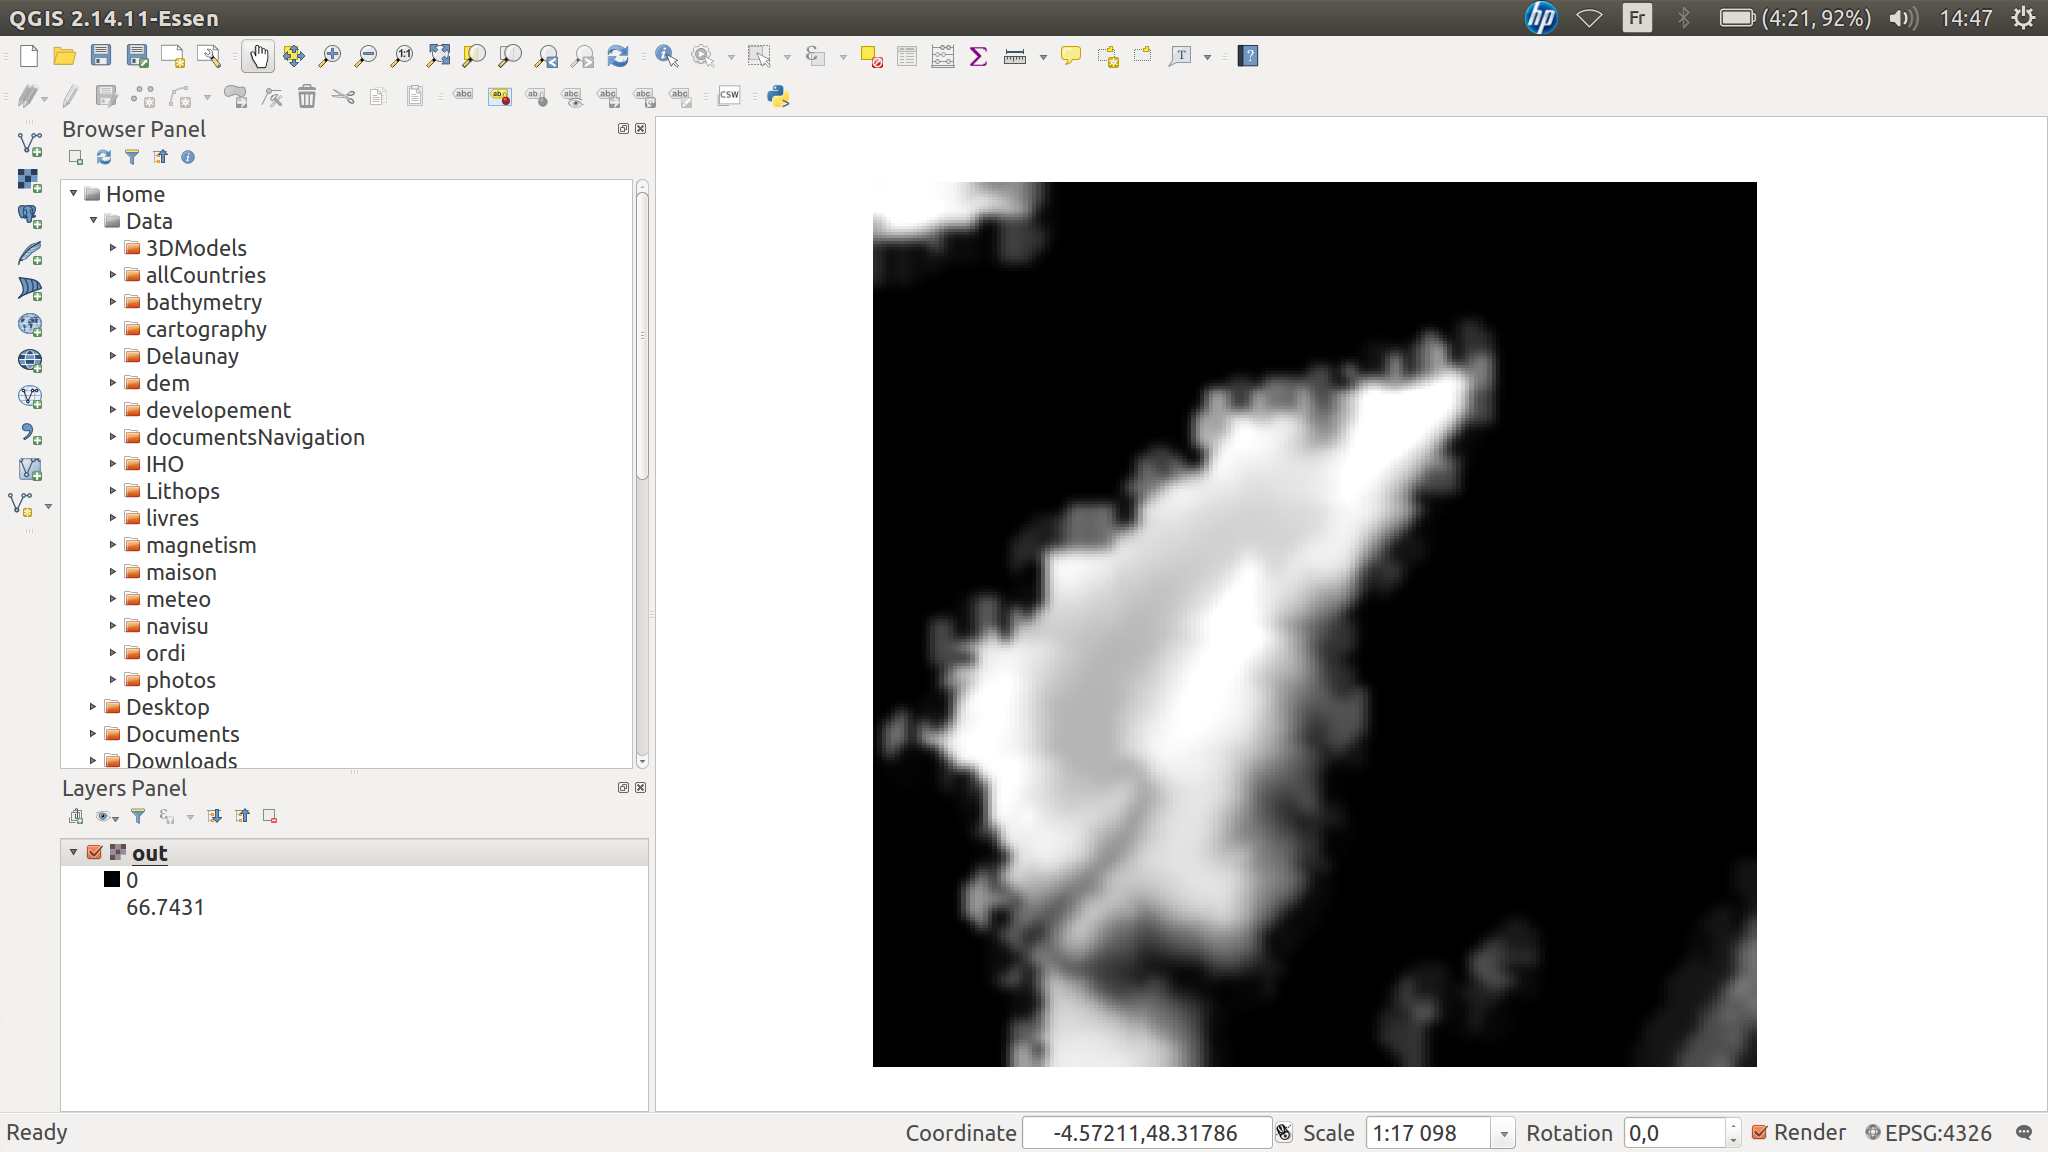
\includegraphics[width=15cm]{images/stl/geoTif.png}
	}
	\begin{figure}[ht]
		\caption{\label{kml}\textit{Export des donn�es en GeoTiff, visualisation QGis}}
	\end{figure}
\end{center}
%%%%%%%%%%%%%%%%%%%%%%%%%%%%%%%%%%%%%%%%%%%%%%%%%%%%%%%%%%%%%%%%%
\section{Export ASC}
\section{Export Shapefile}






%%%%%%%%%%%%%%%%%%%%%%%%%%%%%%%%%%%%%%%%%%%%%%%%%%%%%%%%%%%%%%%%%
\chapter{Utilisation du logiciel}
%%%%%%%%%%%%%%%%%%%%%%%%%%%%%%%%%%%%%%%%%%%%%%%%%%%%%%%%%%%%%%%%%

\section{Interface utilisateur}
%%%%%%%%%%%%%%%%%%%%%%%%%%%%%%%%%%%%%%%%%%%%%%%%%%%%%%%%%%%%%%%%%
\begin{center}
	\framebox[1\width]{
		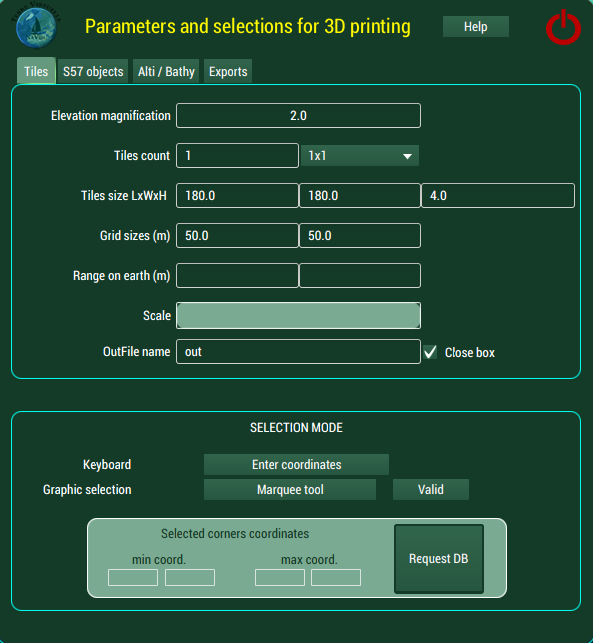
\includegraphics[width=16cm]{images/utilisation/tilesSTL.png}
	}
	\begin{figure}[ht]
		\caption{\label{menu}\textit{Menu principal : choix des param�tres g�n�raux}}
	\end{figure}
\end{center}

%%%%%%%%%%%%%%%%%%%%%%%%%%%%%%%%%%%%%%%%%%%%%%%%%%%%%%%%%%%%%%%%%
%%%%%%%%%%%%%%%%%%%%%%%%%%%%%%%%%%%%%%%%%%%%%%%%%%%%%%%%%%%%%%%%%
\begin{center}
	\framebox[1\width]{
		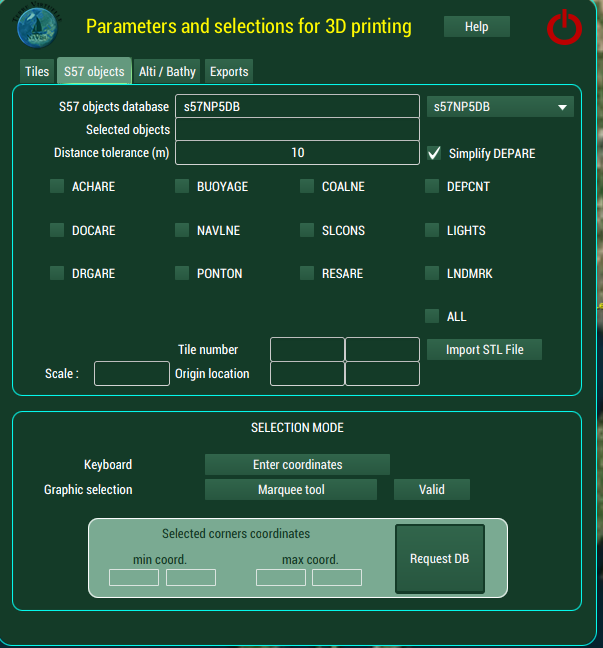
\includegraphics[width=16cm]{images/utilisation/s57STL.png}
	}
	\begin{figure}[ht]
		\caption{\label{menu}\textit{Choix des objets S57 � repr�senter}}
	\end{figure}
\end{center}

%%%%%%%%%%%%%%%%%%%%%%%%%%%%%%%%%%%%%%%%%%%%%%%%%%%%%%%%%%%%%%%%%
%%%%%%%%%%%%%%%%%%%%%%%%%%%%%%%%%%%%%%%%%%%%%%%%%%%%%%%%%%%%%%%%%
\begin{center}
	\framebox[1\width]{
		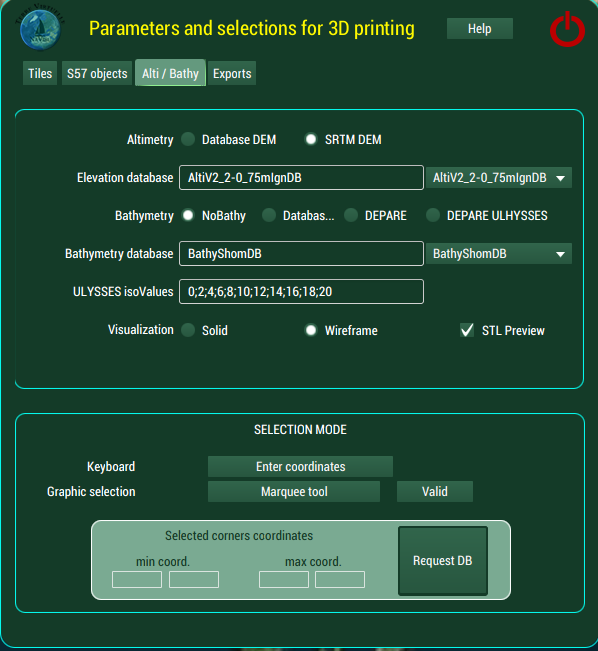
\includegraphics[width=16cm]{images/utilisation/altiBathySTL.png}
	}
	\begin{figure}[ht]
		\caption{\label{menu}\textit{Choix des mod�les num�riques de terrain � repr�senter}}
	\end{figure}
\end{center}

%%%%%%%%%%%%%%%%%%%%%%%%%%%%%%%%%%%%%%%%%%%%%%%%%%%%%%%%%%%%%%%%%
%%%%%%%%%%%%%%%%%%%%%%%%%%%%%%%%%%%%%%%%%%%%%%%%%%%%%%%%%%%%%%%%%
\begin{center}
	\framebox[1\width]{
		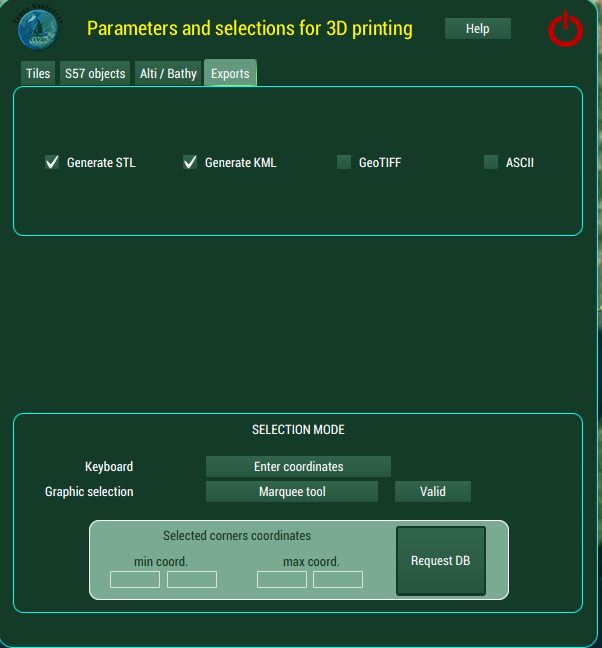
\includegraphics[width=16cm]{images/utilisation/exportSTL.png}
	}
	\begin{figure}[ht]
		\caption{\label{menu}\textit{Choix des formats d'export}}
	\end{figure}
\end{center}

%%%%%%%%%%%%%%%%%%%%%%%%%%%%%%%%%%%%%%%%%%%%%%%%%%%%%%%%%%%%%%%%%
%%%%%%%%%%%%%%%%%%%%%%%%%%%%%%%%%%%%%%%%%%%%%%%%%%%%%%%%%%%%%%%%%
\begin{center}
	\framebox[1\width]{
		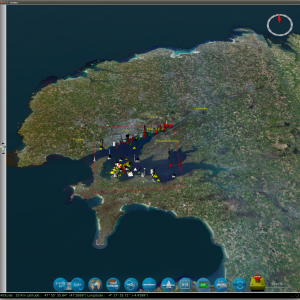
\includegraphics[width=14cm]{images/utilisation/rade_1-300x300.png}
	}
	\begin{figure}[ht]
		\caption{\label{mntAlti}\textit{S�lection d'une zone et des objets recherch�s}}
	\end{figure}
\end{center}
%%%%%%%%%%%%%%%%%%%%%%%%%%%%%%%%%%%%%%%%%%%%%%%%%%%%%%%%%%%%%%%%%
%%%%%%%%%%%%%%%%%%%%%%%%%%%%%%%%%%%%%%%%%%%%%%%%%%%%%%%%%%%%%%%%%
\begin{center}
	\framebox[1\width]{
		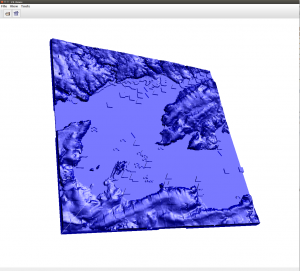
\includegraphics[width=14cm]{images/utilisation/rade-300x271.png}
	}
	\begin{figure}[ht]
		\caption{\label{mntAlti}\textit{S�lection d'une zone et des objets recherch�s : r�sultat en STL}}
	\end{figure}
\end{center}
%%%%%%%%%%%%%%%%%%%%%%%%%%%%%%%%%%%%%%%%%%%%%%%%%%%%%%%%%%%%%%%%%
\chapter{Les publications}
%%%%%%%%%%%%%%%%%%%%%%%%%%%%%%%%%%%%%%%%%%%%%%%%%%%%%%%%%%%%%%%%%
%%%%%%%%%%%%%%%%%%%%%%%%%%%%%%%%%%%%%%%%%%%%%%%%%%%%%%%%%%%%%%%%%
\chapter{Les r�sultats}
%%%%%%%%%%%%%%%%%%%%%%%%%%%%%%%%%%%%%%%%%%%%%%%%%%%%%%%%%%%%%%%%%

%%%%%%%%%%%%%%%%%%%%%%%%%%%%%%%%%%%%%%%%%%%%%%%%%%%%%%%%%%%%%%%%%
\chapter{Les futurs travaux}
%%%%%%%%%%%%%%%%%%%%%%%%%%%%%%%%%%%%%%%%%%%%%%%%%%%%%%%%%%%%%%%%%

\section{Exploration des d�tails de bathym�trie}
LIDAR

\section{Int�gration des donn�es Open Street Building}


	\newpage
	\label{fin}
	
	% ------------------------------------------------------------------------------
\end{document}
